\documentclass[lettersize]{sig-alternate-konrad}
\usepackage{listings}
\usepackage{times}  % Use Adobe Times font set
\usepackage{url}
\usepackage{textcomp}
\usepackage{graphicx} 
\usepackage{color}
\usepackage{multirow}

\setlength{\abovecaptionskip}{-0.05in}
\setlength{\belowcaptionskip}{-0.05in}

\pagestyle{empty}

\begin{document}

\conferenceinfo{SenSys'08,} {November 5--7, 2008, Raleigh, North Carolina, USA.} 
\CopyrightYear{2008}
\crdata{978-1-59593-990-6/08/11}

\title{{\ttlfnt Lance: Optimizing High-Resolution Signal Collection
in Wireless Sensor Networks}}
\author{{\aufnt Geoffrey Werner-Allen, Stephen Dawson-Haggerty$^\star$, and Matt
Welsh} \\
{\affaddr School of Engineering and Applied Sciences, Harvard
University, Cambridge, MA 02138} \\
{\affaddr $^\star$ University of California, Berkeley, Berkeley, CA 94720} \\
{\affaddr \{werner,mdw\}@eecs.harvard.edu, stevedh@cs.berkeley.edu} \\
{\affaddr \texttt{http://fiji.eecs.harvard.edu/Lance}}}
\maketitle

\maketitle
\thispagestyle{empty}

\subsection*{Abstract}
An emerging class of sensor networks focuses on reliable 
collection of high-resolution signals from across the network.
In these applications, the system is capable of acquiring more 
data than can be delivered to the base station, 
due to severe limits on radio bandwidth and energy.
Moreover, these systems are unable 
to take advantage of conventional approaches to in-network data
aggregation, given the high data rates and need for raw signals.
These systems face an important challenge: how to
maximize the overall value of the collected data, subject to resource constraints.

In this paper, we describe {\em Lance}, a general approach to
bandwidth and energy management for reliable data collection in wireless
sensor networks. Lance couples the use of optimized, data-driven 
reliable data collection with a model of energy cost for extracting 
data from the network. Lance's design decouples resource allocation 
mechanisms from application-specific policies, enabling flexible 
customization of the system's optimization metrics.

We describe the Lance architecture in detail, demonstrating its
use through a range of target applications and resource management
policies. We present an extensive study driven by both 
real and synthetic data distributions, through simulations and runs
on a large sensor testbed.  We show that Lance maximizes 
the value of the collected data under a range of resource 
constraints, achieving near-optimal allocation of radio bandwidth and
energy. Finally, we present results from a real sensor network
deployment at Tungurahua volcano, Ecuador, in which Lance was used to
drive data collection for an eight-node network collecting seismic and
acoustic signals from the active volcano.  


\category{C.2.4}{Distributed Systems}{}
\category{C.3}{Special-Purpose and Application-Based
Systems}{Real-time and embedded systems}
\vspace{-0.1in}
\terms{Design}
\vspace{-0.1in}
\keywords{Wireless Sensor Networks, Data Collection, Resource
Management}

\section{Introduction}

Many sensor network applications involve the acquisition
of high-resolution signals using low-power wireless sensor nodes. Examples
include monitoring acoustic, seismic, and vibration waveforms in
bridges~\cite{ggb-ipsn07}, industrial equipment~\cite{intel-northseasensys}, 
volcanoes~\cite{volcano-osdi06}, and animal
habitats~\cite{girod-ipsn07,enviromic}.  These systems all attempt to acquire
high data-rate (100~Hz or higher), high-fidelity data across the network,
subject to severe constraints on radio bandwidth and energy usage.

Given these constraints, it is typically not possible to acquire
continuous waveforms from all nodes.  As a result, applications strive
to acquire the most ``interesting'' signals, such as a marmot call or
earthquake, and avoid wasting resources on ``uninteresting'' signals.
Currently, these resource-management decisions are made on an {\em ad
hoc} basis for each application, often resulting in suboptimal solutions
that can consume excessive bandwidth or lose data.  We argue that all
of these applications would benefit from a general approach to managing
resources that optimizes the application-specific value of the
data acquired by the network.

Optimizing reliable data acquisition requires a coordinated approach
to managing both limited energy capacity and severely constrained
radio bandwidth. Depending on the sampling rate and
resolution, downloading signals may take longer than real time;
while low-power 
sensor node radios obtain single-hop throughput of about 100~Kbps, the
the best reliable protocols achieve less than 
8~Kbps for a single transfer over multiple hops~\cite{flush-sensys07}. 
Likewise, to achieve long lifetimes in the field, the energy cost of 
downloading a signal from the network must be carefully considered. 
The fundamental challenge is how to best direct these limited network
resources to acquire the most valuable data to the application.

This paper presents {\em Lance}, a general approach to bandwidth and energy
management for reliable signal collection in wireless sensor networks. In
Lance, each node acquires data at potentially high rates. For each
application data unit (ADU), each node generates a concise ADU {\em summary},
which is periodically sent to the base station and used to compute a ADU {\em
value}.  Lance computes an ADU {\em download schedule} based on these values,
and uses a reliable transfer protocol to download ADUs according to this
schedule.

Energy usage and battery lifetime are major concerns for long-term
sensor network deployments. 
Lance incorporates a {\em cost estimator} that
predicts the energy cost for reliably
downloading each ADU from the network. We describe a novel energy cost
estimation algorithm that uses information on the network topology to 
determine the energy cost at the sensor node hosting the ADU as well
as intermediate nodes impacted by the multihop transfer protocol. 
Information from the cost estimator is used to adjust the download
schedule for ADUs, allowing Lance to target a battery lifetime for 
the network by load-balancing download operations in a manner that
adheres to an energy schedule.

Lance incorporates a general framework for managing bandwidth and
energy that decouples the mechanism for prioritizing resource allocation from
the application-specific policies used to assign ADU values.
This is accomplished through user-supplied {\em policy modules} that
permit a range of sophisticated prioritization policies to be
tailored for specific applications. Policy modules allow Lance to
target a broad range of optimization metrics, including node-local and
network-wide value maximization, lifetime targeting, 
and acquiring temporally-
or spatially-correlated data from across the network. 
Policy modules allow the network's behavior to be significantly altered
at the base station, without reprogramming the sensor nodes themselves.

The contributions of this paper are as follows. First, we present the
Lance architecture in detail, which is the first system to provide 
a value-driven bandwidth and energy management framework for 
high-data-rate sensor networks. Second, we describe Lance's policy 
modules, which offer a clean separation of policy and mechanism that 
allows the system to be tailored to a broad range of applications. 
We focus on one application in detail: using Lance to maximize data 
quality for a network of seismic and acoustic sensors deployed at 
an active volcano. Third, we show through detailed simulation 
measurements that Lance achieves {\em near optimal} efficiency 
(greater than 96\% in most cases) under a range of data distributions 
and resource limitations. 
Fourth, we present results from 
an eight-node field deployment of Lance at Tungurahua Volcano, 
Ecuador, demonstrating the system's performance in a real 
field setting and the flexibility of policy modules for 
altering the network's operation following deployment. 

The rest of this paper is organized as follows.
Section~\ref{sec-motivation} presents motivation and related
work. We describe the architecture of Lance in detail in
Section~\ref{sec-architecture} and discuss the use of application-specific
policy modules in Section~\ref{sec-policies}.  Section~\ref{sec-casestudy}
presents a case study of several applications that can make use
of the Lance architecture.  We briefly describe our prototype in
Section~\ref{sec-implementation}.  Section~\ref{sec-evaluation}
presents a detailed evaluation while Section~\ref{sec-deployment}
presents results from our field deployment. Finally,
Section~\ref{sec-conclusions} discusses future work and concludes.

\section{Background and Motivation}
\label{sec-motivation}

Wireless sensor networks are becoming more common for applications
that focus on reliable collection of raw signals at relatively high sampling
rates, as opposed to in-network aggregation of low-data-rate samples.
These applications generally make use of extensive offline analysis 
to study the collected data, and it is often infeasible
or impossible to perform this computation within the network itself.
Even in cases where it is possible to shift computation to the network, a
system designer may wish to extract raw data occasionally for calibration
or testing.  Examples of such applications include structural health
monitoring~\cite{netshm-spots06,ggb-ipsn07,wimms-lynch06}, acoustic
sensing~\cite{vango,vigilnet,girod-ipsn07,enviromic}, distributed camera
networks~\cite{cyclops}, and geophysical monitoring~\cite{volcano-osdi06}.

These systems typically record data to flash at each sensor node 
and make use of a reliable bulk-transfer protocol to collect data at 
a base station. Given that the network is capable of sampling data at
a higher rate than it can be downloaded, it is not possible to 
collect the complete signal from all nodes. 
The system is therefore forced to make
a decision about what data to collect and what to throw away. In most
cases this decision is application-specific: for example, a
volcanologist may be chiefly interested in a specific type of seismic
tremor, and a biologist may be looking for acoustic signatures of a 
specific species of marmot~\cite{girod-ipsn07}. The implication is that
the system must be able to determine the intrinsic {\em value} of
a given signal to determine whether resources should be devoted to 
storing and downloading that signal.

Previous approaches have involved simple mechanisms tailored for 
specific applications. For example, in the
NetSHM~\cite{netshm-spots06,netshm-emnets05} structural monitoring 
system, data collection is 
triggered manually following an excitation of the structure.
Sentri~\cite{ggb-ipsn07} has been used for vibration monitoring at
the Golden Gate Bridge; it is unclear from the paper how sampling and
communication are triggered, but reported experimental results
suggest manual operation. The Reventador volcano monitoring 
system~\cite{volcano-osdi06} used a simple triggering algorithm to detect 
seismic events and initiate reliable transfer to the base station. 
The Intel Predictive Maintenance
system~\cite{intel-northseasensys} performs high-data-rate sampling
staggered over infrequent, periodic collection periods to extend
system lifetime. 
All of these systems involve a tight binding of the {\em mechanisms} 
used to manage storage and bandwidth with their respective 
application-specific {\em policies}.

The typical approach to download management is a FIFO model where downloads
occur in a round-robin fashion across the network once a trigger occurs. In
general, new data may be sampled and stored to flash while a download is
taking place.  Therefore, the trigger frequency, download cycle duration and
the number of nodes in the network all effect the amount of data captured by
such an approach.  For example, the Flush~\cite{flush-sensys07} protocol
achieves only 8~Kbps for a reliable transfer over multiple hops; the
Fetch~\cite{volcano-osdi06} and Straw~\cite{ggb-ipsn07} protocols fare
somewhat worse. The RCRT protocol~\cite{rcrt-sensys07} is designed for a case
where all nodes are transmitting simultaneously to the sink, although this
approach severely limits the obtained per-node throughput. As a result, when
incoming data rates exceed download capacity, FIFO download management can
produce excessive delays between data acquisition and retrieval.

Lance assumes that sensor nodes contain adequate flash storage to buffer
signals prior to download.  While the popular TMote~Sky platform supports a
relatively small 1~MB flash, more recent sensor designs~\cite{shimmer} have
several GB~of flash, and we expect this trend to continue. Rather than
focusing on per-node storage, our primary concern is with limitations on
bandwidth and energy.

Our goal is to develop a general-purpose approach to bandwidth and energy
management that complements a reliable data-collection protocol. Such a
system should have several key properties.  First, it should be {\em
customizable}, allowing different applications to specify their own policies
for storage management and bandwidth prioritization. Second, the system
should target a range of optimization goals. Examples include maximizing
overall data priority, bounding energy consumption, maximizing temporal or
spatial coverage of the collected data, or achieving fairness across sensor
nodes. Third, the system should be decoupled from a specific routing
protocol, reliable collection protocol, or sensor node platform, making it
possible to leverage the system in different settings. 

{\bf Related work:}
Several systems are related to Lance but differ substantially in their
goals and assumptions.  EnviroMic~\cite{enviromic} is a system
designed to support distributed acoustic recording by leveraging the 
collective storage resources of multiple sensor nodes. 
EnviroMic focuses on storage management and load balancing, and
assumes that data will be manually retrieved from sensor nodes
following the deployment. Unlike Lance, EnviroMic is not intended 
for applications with real-time data needs.

ICEDB~\cite{zhang2007icedb} supplies a delay-tolerant and priority-driven
query processor for the CarTel~\cite{cartel} system. While ICEDB
considers bandwidth limitations, it does not consider energy as a
constraint. ICEDB provides SQL extensions allowing queries to assign
both inter- and intra-stream priorities, which are used by the query
processor to manage bandwidth and storage resources. ICEDB also uses a
similar node-level summarization technique to that used by Lance. 

VanGo~\cite{vango} provides an architecture for collecting and processing
high-resolution sensor data on resource-constrained nodes.  VanGo focuses on a
programming model based on a linear filter chain and implementing efficient
signal-processing operations with limited computational power.
WaveScope~\cite{wavescope} and Flask~\cite{flask-tr} are languages for stream
processing applications.  These systems are largely complementary to Lance,
and could be used to process signal data prior to collection, although our
focus is on collecting {\em raw} sensor data from large networks.  These
systems do not attempt to optimize data collection under varying energy and
bandwidth constraints. 

\section{Lance System Architecture}
\label{sec-architecture}

\begin{figure}[t]
\begin{center}
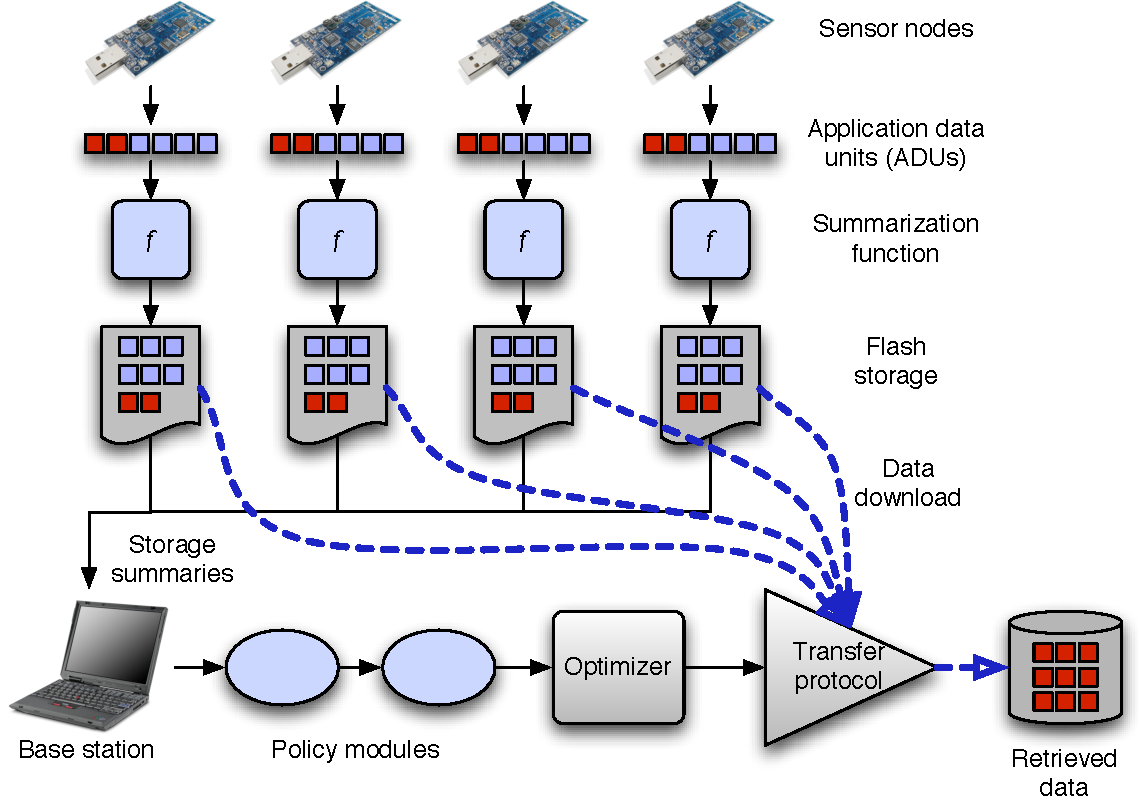
\includegraphics[width=1.0\hsize]{./figs/new-arch.pdf}
\end{center}
\caption{\small {\bf The Lance system architecture.} {\em The
summarization portions are provided by the
application; all other components are generic.}}
\label{fig-architecture}
\end{figure}

This section describes the Lance architecture, introducing a
formal problem definition, design principles, and major system components.
Section~\ref{sec-implementation} covers implementation details omitted here.

\subsection{Problem definition}
\label{sec-problem-definition}

In Lance, the network consists of a set of sensor nodes that continuously
sample and store sensor data into {\em application data units (ADUs)}, which
are the unit of data storage and retrieval.  Each unique ADU $a_i$ consists
of a tuple $\{ i, n_i, t_i, d_i, v_i, \bar{c}_i \}$, 
where $i$ is a unique ADU identifier,
$n_i$ is the node storing the ADU, $t_i$ is a timestamp, and $d_i$ is the raw
sensor data.  We assume that ADUs are of uniform size and that nodes 
have sufficient flash storage to buffer collected signals, so an 
ADU is only evicted from a node's flash once it has been downloaded.
We define the {\em universe} $U$ as the set of all ADUs sampled by the 
network over time. 

Every ADU is assigned an application-specific {\em value} $v_i$ that
represents the application's intrinsic ``utility'' for the data contained
within the ADU.  We make no assumptions about how ADU values are assigned;
the value could be a function of the data itself, the time the data was
acquired, which node sampled the data, data being sampled by other nodes,
and so forth. Lance provides a flexible infrastructure for applications
to define their own value functions through policy modules.

Each ADU has an associated cost $\bar{c}_i$ that represents the energy
requirement to download the ADU from the network.  $\bar{c}_i$ is a vector
$\{ c_i^1, c_i^2, \ldots, c_i^n \}$ where $c_i^j$ represents the estimated
energy expenditure of node $j$ when ADU $i$ is retrieved. The key idea is
that we explicitly model both the energy cost for downloading the ADU from
its ``host'' node $n_i$ and the energy cost for each node along the
routing path from $n_i$ to the base station which must forward packets during
the transfer. In addition, we also model the energy cost to nodes that
overhear transmissions by nodes participating in the transfer.  This energy
cost on intermediate nodes is non-negligible, since reliable transfer
protocols involve a potentially large number of retransmission. However, the
overhearing cost is typically small, since modern low-power MAC protocols
quickly return to sleep when overhearing transmissions to another node.  The
cost vector $\bar{c}_i$ therefore depends on the network topology.

We assume that each node has a battery with a fixed capacity of $C$
joules, and no energy harvesting is performed in the field. 
Without loss of generality, let us assume that $C$ is
identical for all nodes in the network and is known {\em a priori}. 
We define the {\em lifetime target} $L$ as the desired lifetime 
of each node in the network. To meet the lifetime
target, nodes should strive to consume no more than $C/L$ 
joules per unit time on average; we call this the {\em discharge rate} of 
the node. 

The high-level goal of Lance is to download the set of ADUs that
maximizes the total value, subject to the lifetime target. Abstractly,
we define an {\em epoch duration} $\Delta$. Over each epoch, the 
energy consumption of each node must be less than the discharge rate,
that is, $\sum_i \sum_j c_i^j \leq \Delta \times C/L$. 
Determining the optimal set of ADUs to download can be determined by 
solving a multidimensional knapsack problem in which each ADU
represents an item to place in the knapsack with value $v_i$ and 
cost $\bar{c}_i$. The knapsack has $N$ dimensions (where $N$ is the
number of nodes in the network), each of size $\Delta \times C/L$
representing the energy availability over an epoch.
However, calculating the optimal
solution requires {\em a priori} knowledge of all ADUs generated by
the network over time. Clearly, any real system must make use of an
online, heuristic algorithm to approximate the optimal solution.
We discuss and evaluate several different approaches, presenting 
results with respect to the optimal offline solution.

\subsection{Design principles}

Before describing Lance in detail, we first outline several principles 
that guide its design. 

{\em Decouple mechanism from policy.}
We wish to make it easy to adapt Lance to different application
domains by providing a simple set of underlying mechanisms for 
weighing cost and data value that can be tailored 
for different
end-user goals. These core mechanisms should not be tied to any
interpretation of the data stored in an ADU. This approach leads 
to a clean separation of concerns between Lance's resource management
layer and the higher-level policies informing its operation.

{\em Simplicity through centralized control.} In a field deployment setting, 
it is highly desirable for the sensor network to be as simple
as possible, to prevent failures or unexpected behavior due to bugs.
Past deployment experiences have taught us, and others, that 
introducing complex dynamics within the network can lead to a system
that is difficult to understand, debug, or fix in the
field~\cite{volcano-osdi06,volcano-ewsn05}.
To maximize the chances of a successful deployment, 
Lance places most of the control
logic at the base station, treating sensor nodes as slave devices.
This principle makes it easy to change the behavior of the network
at the base station and allows nodes to fail independently without 
affecting the rest of the system. Conventional replication and
failover techniques can be used to bolster the reliability of the 
base station itself.

{\em Low cost for maintenance traffic.} Given limited node energy, 
we wish to reserve as much capacity as possible to support
data collection. This implies that the system
should strive to limit control messages between the base station and
the sensor nodes, as well as internal traffic within the network, as
transmitting packets unnecessarily consumes valuable energy.
This is somewhat at odds with the need for central control,
as the latter could require extensive coordination between 
sensor nodes and the base station; we wish to strike a good balance
between these two conflicting goals.

\subsection{System overview}

Figure~\ref{fig-architecture} provides an overview of the Lance
architecture. Sensor nodes sample sensor data, storing the
data to local flash storage. Each application data unit (ADU)
consists of
some amount of raw sensor data, a unique {\em ADU identifier}, and a 
{\em timestamp} indicating the time that the first sample in the ADU
was sampled. ADU timestamps can either be based on local clocks at
each node, or tied to a global timebase using a time synchronization
protocol such as FTSP~\cite{ftsp}. The size of an ADU should be
chosen to balance the granularity of data storage and download with
the overhead for maintaining the per-ADU metadata. In the applications
we have studied, an ADU stores several seconds or minutes 
of sensor data, not an individual sample. ADUs are stored
locally in flash, which is treated as a circular buffer.

Ideally, nodes would be able to compute the value $v_i$ of an ADU
locally, as the data is sampled. However, since the value might depend
on factors other than the ADU's data, such as data computed at
other nodes. Lance assigns values $v_i$ at the base station,
based on global knowledge of the state of the network. However, this
requires nodes to communicate some low-bandwidth information on the ADU
contents to the base station.  For this purpose, each node applies an
application-supplied {\em summarization function}, computing a 
concise summary $s_i$ of the contents of the ADU as it is sampled.
Nodes periodically send {\em ADU summary} messages to the
base station, providing information on the ADUs they have sampled,
their summaries, timestamps, and other metadata. As a special case,
if a node is able to assign the ADU's initial value directly, this is used
as the summary.

The Lance {\em controller} receives ADU summaries from the network.
The controller also estimates the download cost $\bar{c}_i$ for each
ADU, based on information on network topology as well as a model of
energy consumption for download operations. The ADU summaries and cost
are passed through a series of {\em policy modules}, which provide
application-specific logic to assign the value $v_i$ to each ADU.
The resulting values are passed to the Lance {\em download manager}
which is responsible for performing downloads, using a reliable
data-collection protocol, such as Flush~\cite{flush-sensys07}.

\subsection{Summarization functions}

Lance computes ADU values using two application-provided components.  The
first is the summarization function, described above.  The second component
is a chain of {\em policy modules} executed at the base station which, by
modifying the value for each ADU, can implement a range of
application-specific policies. Since the base station receives ADU summaries
from every node, the policy modules can use global information not available
to individual nodes to make informed bandwidth and energy allocation
decisions.

Lance places two constraints on the on the summarization function. First,
we require that the summary be small (typically a few bytes) to limit the 
overhead for storing and transmitting these values. Second, 
the function must be able to run efficiently on the sensor node as 
ADUs are being sampled.  Otherwise, the exact form of the function is 
entirely application-specific.

As a concrete example, consider a network for downloading seismic events
from an earthquake zone.  One commonly-used measure of
overall seismicity during a time period is the Real-Time Seismic Amplitude
Measurement (RSAM)~\cite{rsam}, which computes the average amplitude
of a seismic signal over some time window (typically 1~to~10~minutes).
This function is simple to compute and reduces a complex seismic waveform
to a single scalar value, with higher values indicating greater seismic
activity.

Another form of summarization is an event detector, which would
produce a nonzero value whenever an event of interest is
contained within the ADU; the summary might also represent the strength
or confidence of the event detection. For example, an acoustic animal
tracking system~\cite{girod-ipsn07} or countersniper localization
system~\cite{shooter-localization} might use a simple trigger-based
summarization function, indicating the detection of a marmot call or
gunshot in the ADU.

\subsection{Cost estimation}
\label{sec-costassignment}

Lance estimates the download energy cost
vector $\bar{c}_i$ for each ADU sampled by the network. 
We assume that nodes are organized into a spanning tree topology
rooted at the base station. The cost is a function of many factors,
including the reliable transport protocol, each node's position 
in the routing tree, radio link quality characteristics, and the 
MAC protocol. 

Given the complex dynamics that can arise during a sensor network's
operation, we opt to use a simple conservative estimate of the energy cost to
download an ADU from a node. Our approach is based on an empirical model that
captures three primitive energy costs involved in downloading an ADU. The
first, $E_d$, represents the energy used to download an ADU from a given node
which includes the energy cost for reading data from flash and sending
multiple radio packets (including any retransmissions) to the next hop in the
routing tree.  The second, $E_r$, represents the energy cost at intermediate
nodes to forward messages during the ADU transfer. The third, $E_o$,
represents the energy cost to nodes that overhear transmissions during a
transfer.  For simplicity, we assume ADUs of fixed size and compute $E_d$,
$E_r$, and $E_o$ based on the time necessary to download an ADU from the
target node.

Using this simple model, we set the elements of the cost vector $\bar{c}_i$ 
as follows. $c_i^n = E_d$ for the node $n$ hosting the ADU, and 
$c_i^m = E_r$ for nodes $m$ along the routing path from
$n$ to the base station. We set $c_i^o = E_o$ for nodes that are
assumed to be within one radio hop of any of the nodes involved in
the transfer. Estimating $\bar{c}_i$ therefore requires
knowledge of the current routing topology. This information 
is readily available: the periodic summary messages, sent to the 
base station by every node, include the node's radio neighbors and 
parent in the routing tree. Cost vectors can be easily recomputed 
whenever the routing topology changes.

To ensure that all nodes meet the lifetime target $L$, Lance models the
energy availability at each node using a token bucket with depth $D$ and fill
rate $C/L$, corresponding to the mean discharge rate.  $D$ is determined by
the target lifetime $L$, the battery capacity $B$ and the background drain
rate $R$.  In general, $D = B - L*R$, so $D$ represents the energy remaining
after the node reserves enough to ensure it can meet its target lifetime at
the background level.

\subsection{Lance optimizer}
\label{sec-lanceoptimizer}

The Lance optimizer is responsible for scheduling ADUs for download,
based on knowledge of the set of ADUs currently stored by the
network, their associated values, and costs. 
ADU download itself is accomplished using a reliable transfer protocol such as 
Fetch~\cite{volcano-osdi06} or Flush~\cite{flush-sensys07}. In our
design, Lance attempts to download a single ADU at a time, in 
order to prevent network congestion, although it may be possible to
download multiple ADUs simultaneously, depending on the network
topology. A download completes either when the entire ADU has been
received or a timeout occurs.

Lance's optimization process attempts to maximize the value of the ADUs
retrieved while adhering to the lifetime target $L$. In essence, we seek a
greedy heuristic approximation of the multidimensional knapsack solution that
would be used by an oracle with complete knowledge of the ADUs sampled by the
network over all time.  The optimizer first excludes ADUs that would involve
nodes without enough energy to perform a download.  That is, if the token
bucket for a given node $m$ has $E(m)$ joules, ADUs for which $E(m) < c_i^m$
are excluded from consideration.  Note that as the bucket fills, the ADU may
become available for download at a later time. We call these ADUs {\em
infeasible}, and the remaining {\em feasible}.

To determine the next ADU to download, the optimizer considers the 
value $v_i$ of each ADU and the its associated cost $\bar{c}_i$.
We consider three {\em scoring functions} that assign a 
download score to each feasible ADU; the ADU with the highest download score
is downloaded next. In the case of ties, an arbitrary ADU is chosen.

The first scoring function, {\em value-only}, simply downloads the feasible
ADU with the highest value $v_i$. Note that {\em value-only} will meet the
network's lifetime target (since only feasible ADUs are considered) but does
not rank ADUs according to cost.  The second scoring function, {\em
cost-total}, assigns the score $\hat{v}_i$ by scaling the value of the ADU by
its total cost: $\hat{v}_i = v_i / \sum_j c_i^j$. The feasible ADU with the
highest score is then downloaded from the network. This approach penalizes
ADUs stored deep in the routing tree, which have a higher overall cost than
those located near the base station. 

The third scoring function, {\em cost-bottleneck}, scales the ADU value $v_i$ 
by the cost to the node that is an energy bottleneck for downloading
this ADU. That is, let $b$ represent the node with the minimum value
of $E(b)$ such that $c_i^b > 0$. {\em cost-bottleneck} sets the score
$\hat{v}_i = v_i / c_i^b$. The intuition behind this scoring function is
that the most energy-constrained node should be considered when
scoring ADUs for download. We evaluate all three scoring functions in 
this paper and show that they yield very different results in terms
of spatial distribution and energy efficiency.

\section{Policy Modules}
\label{sec-policies}

Policy modules provide an interface through 
which applications can tune the operation of the Lance optimizer.
Since policy modules are loaded into the system
at the base station, they can be modified at any time without 
necessitating reprogramming of the sensor nodes themselves.
In this section we provide a general discussion of policy modules and
provide a series of examples of various policies that can be implemented
through this feature. 

\subsection{Definitions}

A policy module is an application-supplied function that takes as input an
ADU summary tuple $a_i = \{ i, n_i, t_i, d_i, \bar{c}_i, s_i, v_i \}$ and
produces a new tuple $a'_i$ with a possibly modified value $v'_i$.  Policy
modules run at the base station, can maintain internal state, and operate
with global knowledge of the ADUs stored in the network. 

A series of policy modules $\{m_1, m_2, ... m_n\}$ are composed into a 
linear chain, which is passed the 
ADU information extracted from the ADU summary messages received at
the base station. The first policy module in the chain is responsible
for assigning the initial value $v_i$ to the ADU based on the summary 
information $s_i$ calculated by the sensor node. 
The final ADU value produced by the chain is used as input to 
Lance's optimizer for the purpose of scheduling ADUs for download.

Lance requires that policy modules be efficient in that
they can process the stream of ADU summaries received from the
network in real time. In practice this is not difficult to accomplish,
as the rate of ADU summary reception is modest, and the base
station (typically a PC or laptop) is assumed to have adequate
resources. For example, a 100-node network with an ADU size of 60~sec 
would receive an ADU summary every 600~msec. Typical policy modules
take a small fraction of this time to run. 

One of the main benefits of policy modules is that they permit 
significant changes to the network's behavior {\em without requiring
changes to the node-level summarization function}. Changing the
latter would typically involve reprogramming sensor nodes. 
In the field, it is often undesirable to reprogram the network 
except when absolutely necessary, and in many cases it is difficult to 
reach sensor nodes physically once deployed. Although systems such as 
Deluge~\cite{deluge} permit over-the-air reprogramming, 
any changes to the sensor node software could result in unexpected
failures that can be very difficult to debug without manual intervention. 
On the other hand, introducing new policy modules at the base station 
is relatively straightforward, and can be quickly reversed without 
risking sensor node failures. 

\subsection{Example policy modules}
\label{sec-example-policies}

\begin{figure}[t]
\begin{center}
\begin{small}
\begin{tabular}{|l|l|} \hline
{\em Policy module} & {\em Description} \\ \hline
{\tt filter} & Set ADUs below threshold to zero value \\
{\tt boost} & Set ADUs above threshold to max value \\
{\tt timespread} & Dilate ADU values across time \\
{\tt spacespread} & Dilate ADU values across space \\
{\tt adjust} & Add or subtract offset to ADU value \\
{\tt smooth} & Apply low-pass filter to remove noise \\
{\tt debias} & Median filter DC debiasing \\
{\tt correlated} & Boost values for correlated events \\
{\tt costfilter} & Filter ADUs above cost threshold \\ \hline
\end{tabular}
\end{small}
\end{center}
\caption{\small {\bf Standard policy modules provided by Lance.}}
\label{fig-policymodules}
\end{figure}

Policy modules can be used to encapsulate a wide range of 
data collection goals, and make it easy to customize Lance's behavior
for specific applications. We provide a standard toolkit of
general-purpose policy modules, summarized in Figure~\ref{fig-policymodules}.
Application developers are free to implement their own modules as well.
By composing modules in a linear chain, it is easy to implement 
various behaviors without requiring a general-purpose ``policy language.'' 

{\bf Value thresholding:}
{\tt filter} is perhaps the simplest example of a policy module that 
filters out ADUs with a value below a given threshold $T$ by
setting their values to zero.
Setting $v'_i = 0$ prevents an ADU from being considered for download by the
optimizer.  This type of filtering can be used to force a drop of low-valued
data. Conversely, the {\tt boost} policy module sets the value for an ADU
above a given threshold to the maximum value, ensuring it will be downloaded
as soon as it is feasible.

{\bf Value adjustment and noise removal:} 
Policy modules can be used to remove the effects of noise or correct 
for node-level value bias, for example, based on poor sensor 
calibration or differences in site response. Moreover, since each node 
computes the ADU summary based only on local sensor data, it may be 
necessary to normalize the ADU values in order to compare 
values across nodes. 

{\tt adjust} adds or subtracts a node-specific offset to each ADU
value to correct for differences in sensor calibration.{\tt smooth}
applies a simple low-pass filter on the raw ADU values to remove
spikes caused by spurious sensor noise.
Likewise, {\tt debias} is intended to remove
sensor-specific DC~bias from the ADU values.
{\tt debias} computes the median ADU value for a given node over 
a time window. It then subtracts the median from each ADU value before 
passing it along to the next module in the chain. 

Likewise, when a sensor network contains
multiple sensors with varying sensitivity, it is natural to
prioritize data from more sensitive instruments. In cases where networks are
deployed to monitor fixed physical phenomena, it may be desirable to
prioritize data from nodes located close to the phenomena being
observed. The {\tt adjust} module can be used to scale
raw ADU values based on a sensor's location, SNR, or other attributes.

{\bf Value dilation:} 
Another useful policy is to dilate a high (or
low) ADU value observed in one ADU across different ADUs sampled
at different times or different nodes. This can be used to achieve
greater spatial or temporal coverage of an interesting signal
observed at one or more nodes. The {\tt timespread} detects ADUs with
a value above some threshold $T$ and 
assigns the same value to those ADUs sampled just before and just
after.
Likewise, the {\tt spacespread} module groups ADUs from across multiple
nodes into time windows and assigns the maximum ADU value to all
ADUs in that window.  Define a window $W(t,\delta)$ as the set of ADUs
such that $t-\delta \leq t_i \leq t+\delta$ where $t$ represents the
center of the window and $\delta$ the window size. {\tt spacespread}
determines the maximum ADU in the window $v^* = \arg_{i \in W} \max v_i$
and sets $v'_i = v^{*}$ for each ADU in $W$. 

{\bf Correlated event detection:}
The {\tt correlated} module is used to 
select for ADUs that appear to represent a correlated
event observed across the entire sensor network. 
{\tt correlated} counts the number of ADUs within a time window
$W(t,\delta)$ with a nonzero ADU value.
If at least $k$ ADUs meet this criterion, we assume that there is 
a correlated stimulus, and the values for all ADUs in 
the set are passed through.  Otherwise, we filter out the ADUs in 
the window by setting $v'_i = 0$ for each ADU in $W$.

As an example of composing policy modules to implement an interesting
behavior, consider the chain
\[
\mathit{filter}(T)\rightarrow\mathit{correlated}(k)\rightarrow\mathit{spacespread}
\]
This policy filters incoming values, rejects time-correlated sets 
with fewer than $k$ ADUs above the threshold, and assigns the max
value across the set to all ADUs. This can be useful in 
systems that wish to perform collection of time-correlated data, but
avoid spurious high-value data from just a few nodes. 
This policy is similar to the volcanic earthquake detector reported 
in~\cite{volcano-osdi06}, expressed as a simple policy module chain.

{\bf Cost-based filtering:}
Lance's optimizer considers both the cost of ADUs as well as their
application-assigned values when making download scheduling decisions.
The cost vector $\bar{c}_i$ is also available to the policy module
chain, allowing policy modules to perform their own adjustments to
the ADU value according to cost, permitting applications to augment 
Lance's own policies for energy scheduling. 
For example, the {\em costfilter} policy module filters out ADUs with
a total energy cost $\sum_j c_i^j$ greater than some threshold; this
ensures that the network avoids expending an arbitrary amount of
energy to download a given ADU (regardless of its data value). 
Policy modules give applications a great deal of control over energy 
usage to complement Lance's own energy scheduling policy.

\section{Application case studies}
\label{sec-applications}
\label{sec-casestudy}

In this section, we present several case studies of how Lance can
benefit different application domains. We describe our use of Lance in
a geophysical monitoring sensor network in detail, and discuss its use for
limb motion analysis, structural monitoring, and animal habitat
monitoring. All of these applications share the challenges that Lance was 
designed to address: the need for reliable data collection with 
limited bandwidth and storage. 

\subsection{Geophysical monitoring}

Wireless sensor networks can greatly benefit geophysical monitoring
applications, such as seismic and acoustic data collection at fault
zones~\cite{ucla-seismic} and volcanoes~\cite{volcano-osdi06}. Low-power
wireless sensors are highly desirable in these settings, where sensors must
be carried to a deployment site by hand and often cannot be manually serviced
once deployed. 

The goal is to deploy a wireless array of sensors for 
monitoring both seismic and infrasonic (low-frequency acoustic)
signals, including earthquakes, tremor, and volcanic eruptions. 
Depending on the level of seismic or infrasonic activity, the network 
might record dozens of events an hour, with each event typically lasting 
less than 60~sec (although long-period tremor events can last minutes 
or hours). 

As an example, in our previous work on volcano monitoring at
Reventador~\cite{volcano-osdi06}, each sensor node continuously sampled two
channels of seismic and acoustic data at 100~Hz per channel with a resolution
of 24~bits/sample. Raw data was stored to the node's flash memory as a
circular buffer.  An event-detection algorithm running on each node would
send an event report to the base station whenever an interesting seismic
signal was detected. If the base station received enough event reports within
a short time window, it would initiate a round-robin download of the last
60~sec of data from each node.  Although this system was successfully
deployed, it exhibited several deficiencies which led to a significant loss
of data~\cite{volcano-osdi06}. 

The first problem is that the decision used to download a given signal 
was based on a simplistic binary approach, based on the event-detection 
algorithm running on each node. As a result, the system could not 
prioritize certain events over others. The event-detector logic used 
a simple threshold scheme, and as reported in~\cite{volcano-osdi06}, 
the threshold was set too low, causing the network to trigger on less 
than 5\% of the actual seismic events.

The second problem was that following each trigger, the network 
initiated a {\em nonpreemptive} download from every node in the
network in a round-robin fashion. This policy caused 
the system to devote resources to downloading small precursor earthquakes 
that immediately preceded larger eruptions~\cite{volcano-osdi06}. 
As a result, many such larger events were not captured. 

Finally, our previous system made no attempt to manage energy. 
As a result, the expected lifetime of the
network is only about a week (using D-cell batteries), necessitating
frequent battery changes over a long deployment.
Clearly, this system could benefit from a prioritized approach to
download management that also considers energy costs to increase
lifetime.

\subsubsection{Adaptation to Lance}

To address these problems, we reimplemented our previous volcano
monitoring system using Lance. Many of the components of the original system,
such as multihop routing, time synchronization, reliable download
protocol, and flash storage interface, remained unchanged. 
The node-level event detector was replaced by an ADU summarization function,
as described below. The base station code for responding to
correlated events was replaced with Lance's optimizer and
policy modules. Our deployment of the completed system at Tungurahua
volcano in August 2007 is discussed in Section~\ref{sec-deployment}.

\subsubsection{Summarization functions}
\label{sec-casestudy-nuc}

The original system was intended to detect correlated seismic
events from across the network and download data from all nodes,
regardless of whether every node detected the event. This was based
on a simple event detector that computes two exponentially-weighted
moving averages (EWMA) of the seismic signal, with different gain
settings; one EWMA represents the short-term average and the other
the long-term average. When the ratio between these two averages
exceeds a threshold, an event detection message is sent to the base 
station. Subsequent triggers are suppressed for a short duration
afterwards.

This policy is straightforward to implement in Lance by using the ``ratio of
two averages'' as the node-level summarization function.  Rather than
performing thresholding at the node level, we report the maximum ratio over
the ADU as its value, allowing Lance to prioritize different events. The base
station's policy modules are configured as shown in
Section~\ref{sec-example-policies}, using a chain of {\tt filter}, {\tt
correlated}, and {\tt spacespread} to implement the equivalent of the event
triggering policy used in the original system. Note that the Lance version of
the system differs from the original in that download management is
value-driven rather than FIFO. Also, Lance can download ADUs from different
events out of order, avoiding the nonpreemptive download problems of the
earlier system.

While our original system was designed to capture short earthquakes,
were also interested in determining whether Lance could be used to
capture different types of volcanic activity. For this, we make use of
the Real-Time Seismic Amplitude Measurement (RSAM)~\cite{rsam}, which
computes the average seismic amplitude over a given time window. 
Intuitively, RSAM measures 
the total amount of ground shaking caused by earthquakes and tremor,
and is often used by volcano
observatories to characterize the overall level of seismic activity.

Different summarization functions and policy modules can be used to implement
a wide range of geophysical monitoring systems with Lance. For example, a
hazard monitoring system could be configured to periodically report RSAM
values for all sensor nodes and download only the strongest events for
further analysis. By limiting downloads to those ADUs with RSAM above some
threshold, energy can be saved. In contrast, a scientific study that wishes
to perform earthquake localization~\cite{aki-richards-80} or tomographic
inversion~\cite{lees-lindley-94} would prefer to download only small
earthquakes with clearly delineated onsets, which can be used to determine
the velocities of seismic waves. Likewise, a researcher studying explosive
events would prefer to download only seismic events with a corresponding
infrasonic component, since non-explosive earthquakes should not generate any
infrasound.

\subsection{Other application domains}

We believe that Lance can be used to benefit many applications that make use
of high-resolution signals delivered over a bandwidth-limited wireless
network. These applications require high data rates, precluding continuous
data collection, and rely on classification techniques to determine which
signals to download. Two examples are given below.

{\bf Structural monitoring:}
Structural monitoring systems collect vibration
waveforms from a building, bridge, or other structure in order to
study structural properties and seismic response.
In previous systems~\cite{netshm-emnets05,ggb-ipsn07}, data collection
has been triggered manually or on a simple periodic schedule. Instead,
Lance can be used to prioritize signals following an earthquake or 
forced excitation of the structure, similar to the EWMA and RSAM
functions described earlier. To save energy, the system could choose a
subset of nodes from which to download data to achieve a good spatial
distribution across the structure. The size of the subset could be
chosen depending on the strength of the excitation. In addition, 
policy modules can be used to perform periodic downloading of ADUs 
from each sensor for calibration, as well as to determine whether 
each sensor is still functioning properly.

{\bf Animal habitat monitoring:}
Habitat monitoring applications that deploy high-bandwidth sensors, such as
microphones or cameras, are good candidates for prioritized data extraction. 
An example application may attempt to download interesting audio signals
facilitating offline species classification or 
localization~\cite{girod-ipsn07}. The summarization function could
involve either a triggered event detector, an audio waveform
classifier, or motion detector from a series of camera images~\cite{cyclops}.

At the base station, policy modules can use offline knowledge of node
positions to modify the initial ADU value. One approach might enhance
spatial coverage by prioritizing data collection from nodes nearby the
source of the signal. Another could reject noise by deprioritizing signals
detected by only one node. For example, if fewer than three nodes
report an audio event, it is impossible to perform acoustic
localization and Lance need not waste bandwidth on the signal.
Policy modules can take other metrics into account as well, 
such as the SNR of the recorded signal or the time of day (e.g.,
reducing confidence in camera images taken at night).

\section{Prototype Implementation}
\label{sec-implementation}
\label{sec-implementation-nsm}

We have implemented Lance in TinyOS 2.x~\cite{tinyos-asplos00} for 
TMote~Sky and iMote2 sensor nodes. The TMote~Sky features a
1~MB flash memory (ST~M25P80) divided into 16~sectors of 64~KB each.
Our current prototype matches the ADU size to the sector size to
simplify storage management, but this is not a fundamental limitation
in the design. Sensor nodes participate in a multihop spanning-tree 
protocol rooted
at the base station; we use the Collection Tree Protocol provided with
TinyOS~2.0 for this purpose. Nodes send a periodic storage summary to the
base station. To improve reliability, we use a
sliding window approach in which each summary includes information on
the last 5~ADUs recorded by the node. The node prioritization function
is implemented as an application-supplied NesC component conforming to
a simple API. Our prototype uses our own Fetch~\cite{volcano-osdi06}
reliable transfer protocol, although it would be straightforward to
replace this with another protocol such as Flush~\cite{flush-sensys07}.

The Lance download manager runs at the base station and receives
data from the network via a ``gateway node'' connected to the base
station by a serial cable or radio modem.  The download manager is 
implemented in Perl and makes use of several external utilities for
reading and parsing storage summary packets and sending download
requests to the network. Policy modules are implemented as separate
UNIX processes (which can be in any language; we typically use Perl) 
that read storage summaries on {\tt stdin} and produce modified
storage summaries on {\tt stdout}. A simple configuration script is
used to compose multiple policy modules into a pipe. We find that
using standard scripting languages and UNIX utilities makes it very
easy to implement a range of policy modules.
A suite of Python utilities for logging, data visualization, and 
managing the network through a GUI are also provided.
\vspace{0.2in}
\section{Evaluation}
\label{sec-evaluation}

\begin{figure*}[t]
\begin{center}
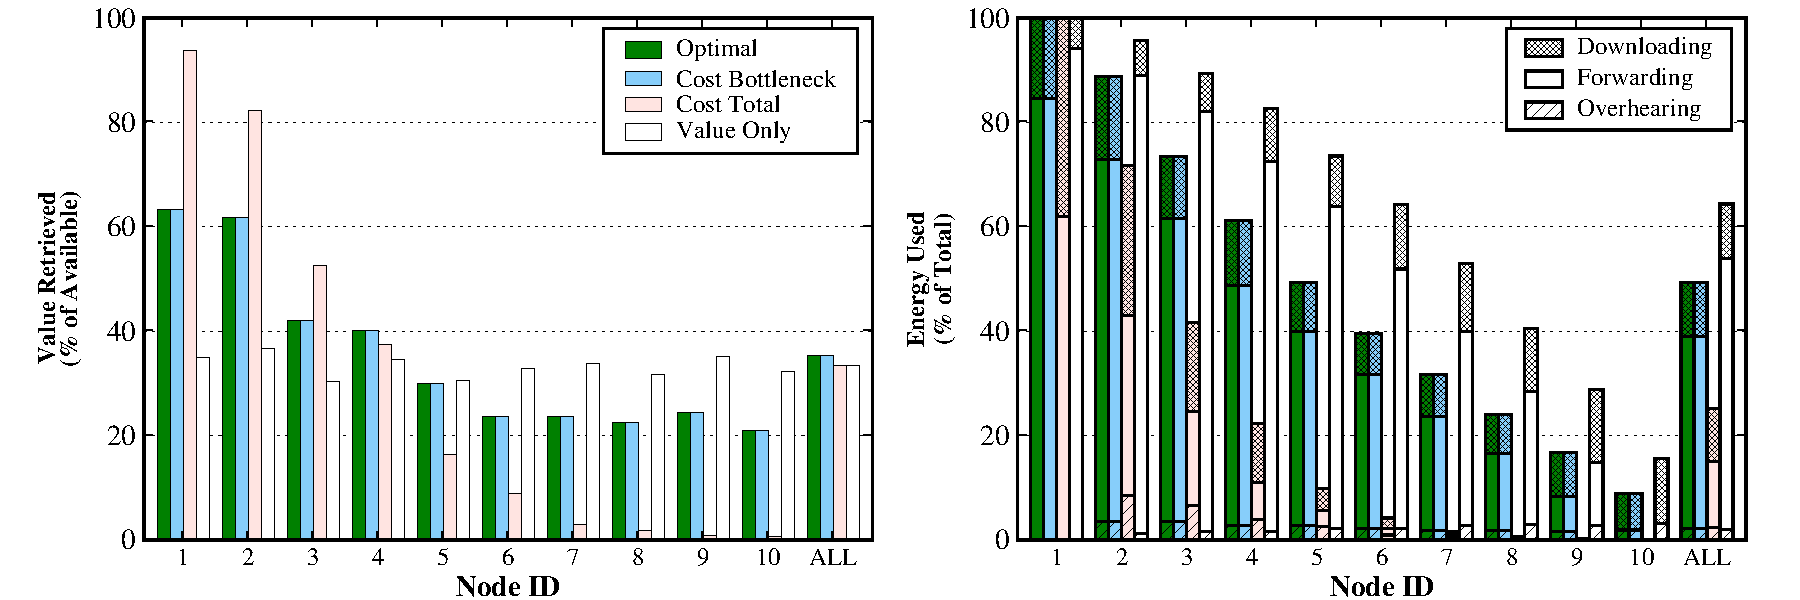
\includegraphics[width=1.0\hsize]{./figs/gwa/linear/BOTH.pdf}
\end{center}
\caption{\small {\bf Per-node distribution of ADU value and energy
usage for the linear simulation experiment.} 
{\em The top graph shows the amount of
data value downloaded from each node, while the bottom graph breaks down the
amount of energy used by each node into the downloading, routing and
overhearing components. Node~1 is closest to the base station.}}
\label{sec-eval-figlinear}
\end{figure*}

\begin{figure}[t]
\begin{center}
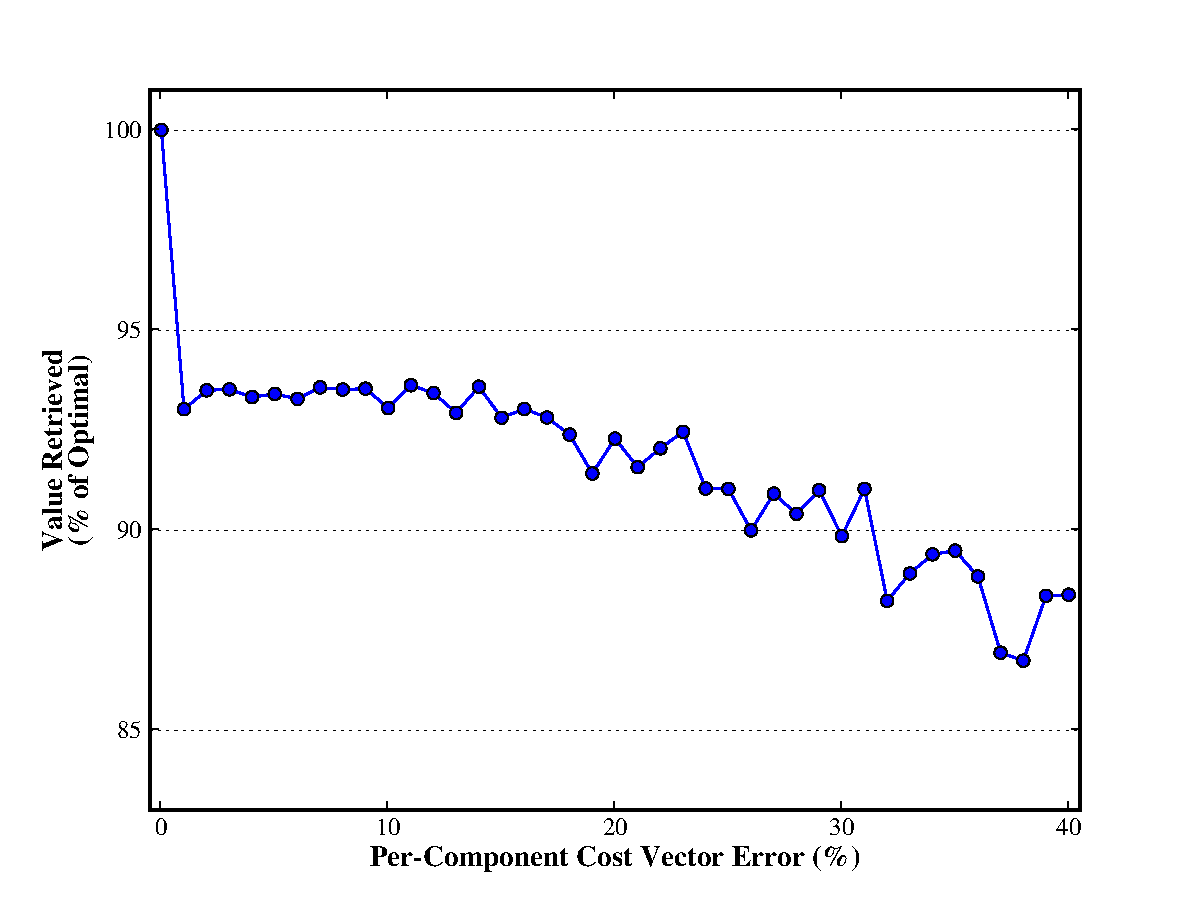
\includegraphics[width=1.0\hsize]{./figs/gwa/error/ERROR.pdf}
\end{center}
\caption{\small {\bf Effect of cost vector error on optimality.} 
{\em The
optimization process is guided by the cost vectors, but predicting the energy
cost of operations before they are performed can be difficult.  Here we show
the impact of introducing a degree of error into the cost vectors used by the
optimizer.  As can be seen, we can tolerate a relatively high degree of
error, as long as the shape of the cost vector does not change.}}
\label{sec-eval-figerror}
\end{figure}

This section presents a careful evaluation of Lance conducted along several
lines.  Using a high-level system simulator and synthetic data sets, we
evaluate the three scoring functions described in
Section~\ref{sec-lanceoptimizer}. We motivate our use of the
\emph{cost-bottleneck} scoring function and demonstrate that it performs
better than simpler alternatives.  Next, we look at the impact of varying
parameters such as download bandwidth and network lifetime, as well
as the impact of errors in the cost vectors.
We also present results from experiments run on a 50-node sensor 
network testbed using realistic data sets.

\subsection{Metrics and methodology}

\begin{figure}[t]
\begin{center}
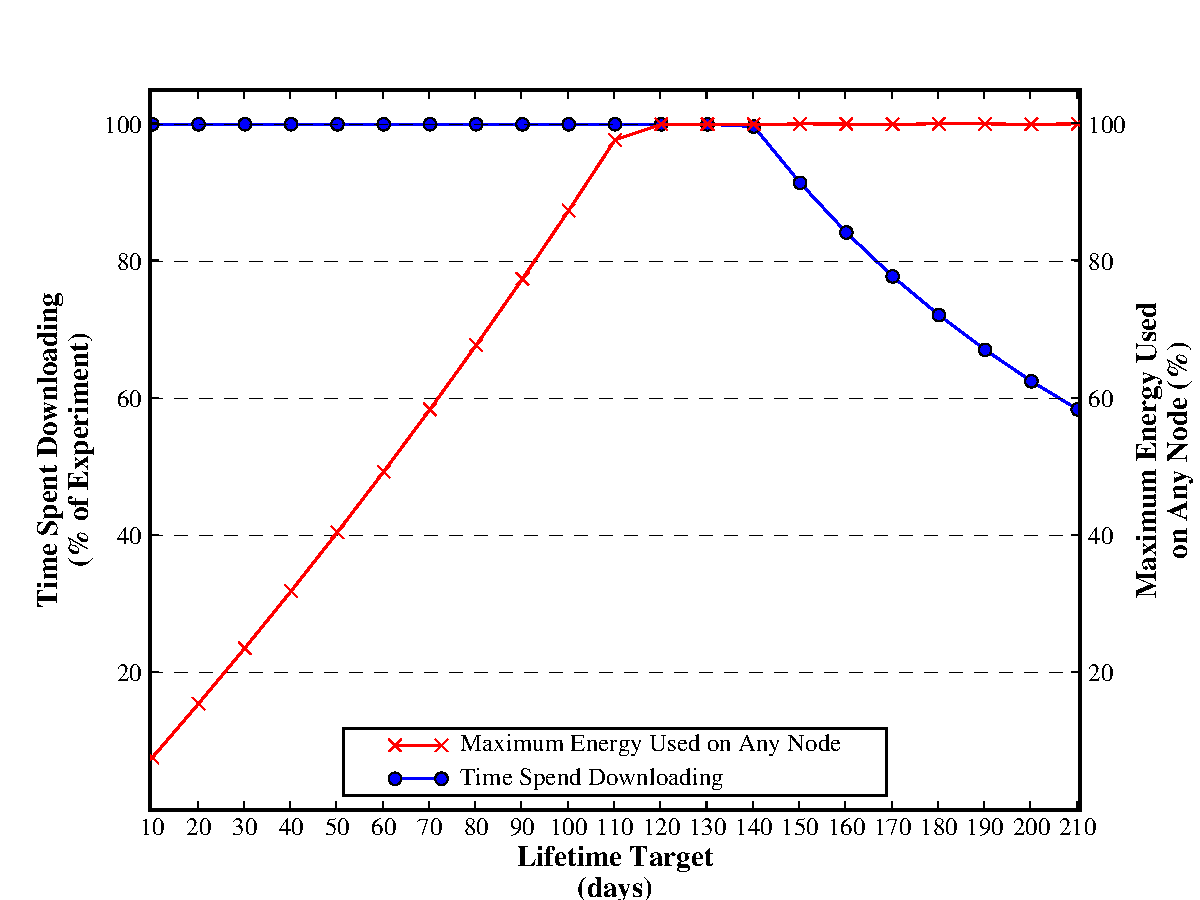
\includegraphics[width=1.0\hsize]{./figs/gwa/crossover/BANDWIDTHVENERGY.pdf}
\end{center}
\caption{\small {\bf Crossover between bandwidth and energy constraint
dominance as lifetime is varied.} 
{\em This graph shows the transition between bandwidth and energy constrained
regions for an optimal system.  The right axis shows the percent of energy
consumed by the most highly-drained node, and the left axis shows the amount
of time spent downloading.}}
\label{sec-eval-crossover}
\end{figure}



As stated in Section~\ref{sec-problem-definition}, the high-level goal of
Lance is to download a set of ADUs maximizing the total value subject to
energy and bandwidth constraints. The {\em optimal} solution is
defined as the solution to the multidimensional knapsack problem,
which yields a set of downloaded ADUs $\mathcal{O} = \{a_1, a_2, ...
a_n\}$ that maximize data value subject to bandwidth and energy
constraints. The total data value of the optimal solution 
$\hat{v}(\mathcal{O}) = \sum_{a_i \in \mathcal{O}} v_i$.
Recall that computing the optimal solution requires {\em a priori} 
knowledge of all of the ADU values sampled by the network over time.
We define {\em optimality} as the fraction of the data value 
downloaded by Lance compared to the optimal solution. That is, given
a set of downloaded ADUs $\mathcal{L}$ with total data value
$v(\mathcal{L})$, we define optimality as 
$v(\mathcal{L}) / \hat{v}(\mathcal{O})$.

We begin by presenting results based on a realistic system
simulator that allows us to quickly vary parameters such as 
ADU data value distribution, network topologies, download speeds,
energy costs, and target lifetimes. We also present results from 
Lance running on MoteLab~\cite{motelab}, a sensor network testbed
deployed over 3~floors of the Harvard EECS building.
Our simulation experiments use
a 10-node linear topology as well as a 25-node realistic tree topology
shown in Figure~\ref{sec-eval-topologies}(a). Both
topologies use per-node ADU download speeds based on empirical 
measurements taken using the testbed. 
In our experiments, the ADU size is 36~KB and each node samples one 
ADU every 60~seconds (or 600~bytes/s of data).

We draw ADU values from several distributions in an attempt to understand
Lance's behavior as the properties of the sampled data change.  Three value
distributions are used: uniform random, exponentially distributed, and Zipf
with exponent $\alpha = 1$.  We also make use of an ADU value distribution
based on a 6~hour seismic signal collected at Reventador Volcano, Ecuador in
2005~\cite{volcano-osdi06}.\\

The energy costs for various operations are modeled as follows.  The
background current drain of each node is set to 2~mA, based on empirical
measurements of a TMote~Sky sensor node performing high-data-rate sampling
and storing to flash.  We also measured the current consumption to download
an ADU from a sensor node, and derived the energy costs for downloading ($E_d
= 17.6$~mA/s), routing ($E_r = 16.9$~mA/s), and overhearing ($E_o = 2$~mA/s).
Our experiments assume that each node can only overhear its parent in the
routing tree; developing more detailed overhearing models is the subject of
future work.  Computing the components of the cost vector for a particular
ADU is done by multiplying the current consumption by the ADU download time
for each node either downloading, routing, or overhearing the transmission.

\subsection{Effectiveness of scoring functions}
\label{sec-eval-heuristics}

\begin{figure}[t]
\begin{small}
\begin{center}
\begin{tabular}{|l|l|ccc|}
\hline
& & \multicolumn{3}{|c|}{Scoring Functions} \\ \hline
& & Value & Cost & Cost \\
Distribution & Lifetime & Only & Total & Bottleneck \\ \hline
\multirow{3}{*}{Uniform} & 4 months & 62.4\% & 90.5\% & \textbf{93.2\%} \\
& 11 months & 43.4\% & 68.0\% & \textbf{96.9\%} \\
& 18 months & 44.6\% & 49.0\% & \textbf{90.0\%} \\ \hline
\multirow{3}{*}{Exponential} & 4 months & 83.9\% & 85.1\% & \textbf{88.0\%}
\\
& 11 months & 70.4\% & 82.0\% & \textbf{93.0\%} \\
& 18 months & 67.2\% & 72.8\% & \textbf{91.2\%} \\ \hline
\multirow{3}{*}{Zipfian} & 4 months & 84.7\% & \textbf{91.4\%} & 87.1\% \\
& 11 months & 63.8\% & 91.1\% & \textbf{96.2\%} \\
& 18 months & 53.1\% & 86.9\% & \textbf{93.8\%} \\ \hline
\end{tabular}
\end{center}
\end{small}
\caption{\small {\bf Optimality of different scoring functions.} 
{\em This table summarizes simulation results evaluating the three 
different scoring functions.  Results are shown for
several different lifetime targets and value distributions. 
{\em cost-bottleneck} out-performs the others 
in almost all cases.}}
\label{sec-eval-table}
\end{figure}

We begin by evaluating the three scoring functions described
Section~\ref{sec-lanceoptimizer}.  We want to see which is the most able to
approximate the optimal solution across a range of target lifetimes
and ADU distributions. As discussed earlier we expected
the \emph{value-only} scoring function, without considering the energy or
bandwidth overhead of downloading each ADU, to consume more 
energy downloading
high-valued ADUs when it could have increased the total data value by
downloading several slightly less-highly valued ADUs with lower costs.  The
\emph{cost-total} scoring function incorporates a notion of cost, but
will tend to favor nodes closer to the base station at the expense
of high-valued ADUs that are more routing hops away. The
\emph{cost-bottleneck} scoring function should strike a balance between 
the two, since it considers only the most significant component 
of the cost vector when ranking ADUs.

Figure~\ref{sec-eval-figlinear} shows simulation results using the 10-node
linear topology with exponentially-distributed ADU values, and a target
lifetime of 3~months.  Nodes are numbered in increasing distance from the base
station.  The graph confirms the intuition behind the scoring function
behavior.  \emph{value-only} downloads roughly equal value from each node,
but fails to match the optimal performance. \emph{cost-total} downloads more
data from nodes near the sink.  \emph{cost-bottleneck} comes close to
matching the optimal solution, retrieving over 99\% of the value retrieved by
the optimal solution.

\begin{figure}[t]
\begin{center}
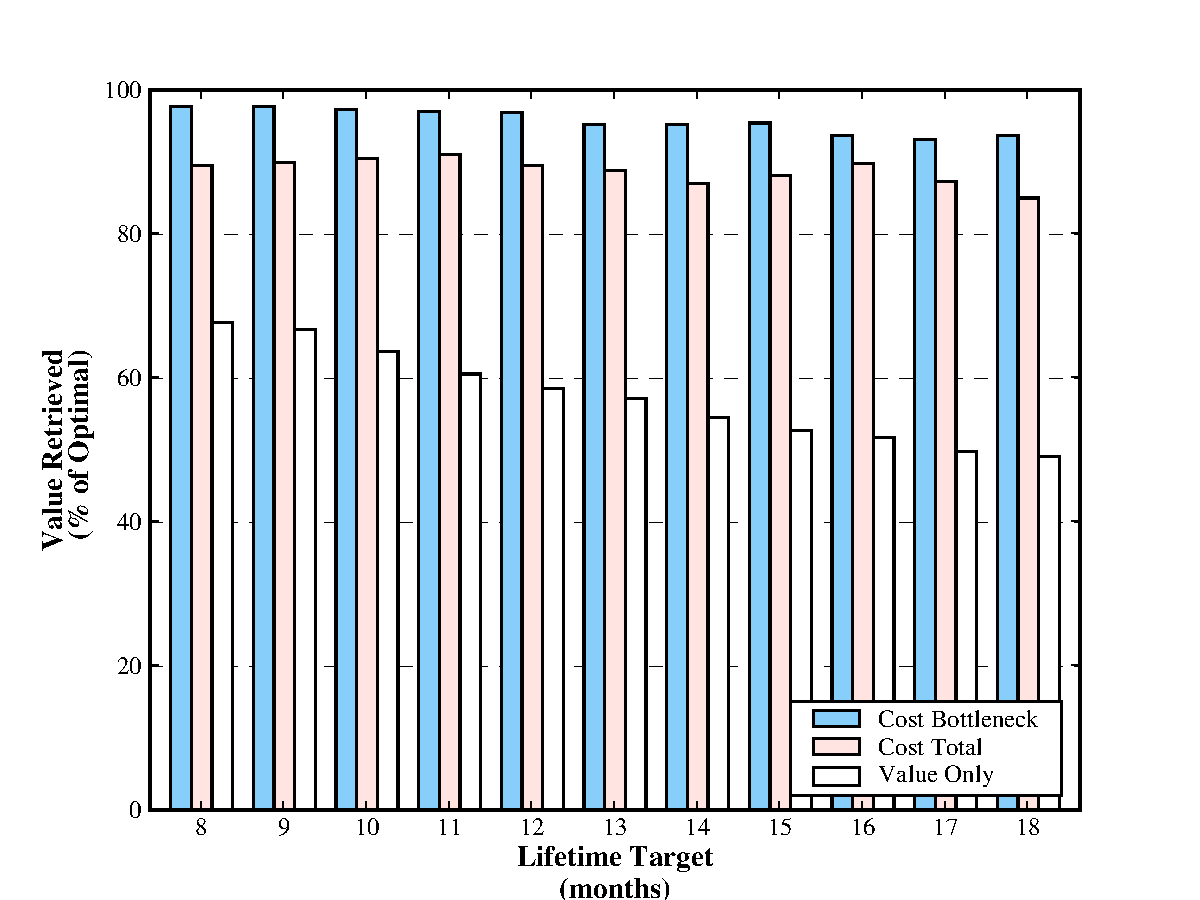
\includegraphics[width=1.0\hsize]{./figs/gwa/zipfian/POLICIES.pdf}
\end{center}
\caption{\small {\bf Scoring function performance on Zipfian distribution.}
{\em The {\em cost-bottleneck} scoring function outperforms the other two
across a range of lifetime targets.}}
\label{sec-eval-zipfian}
\end{figure}

\begin{figure}[t]
\begin{center}
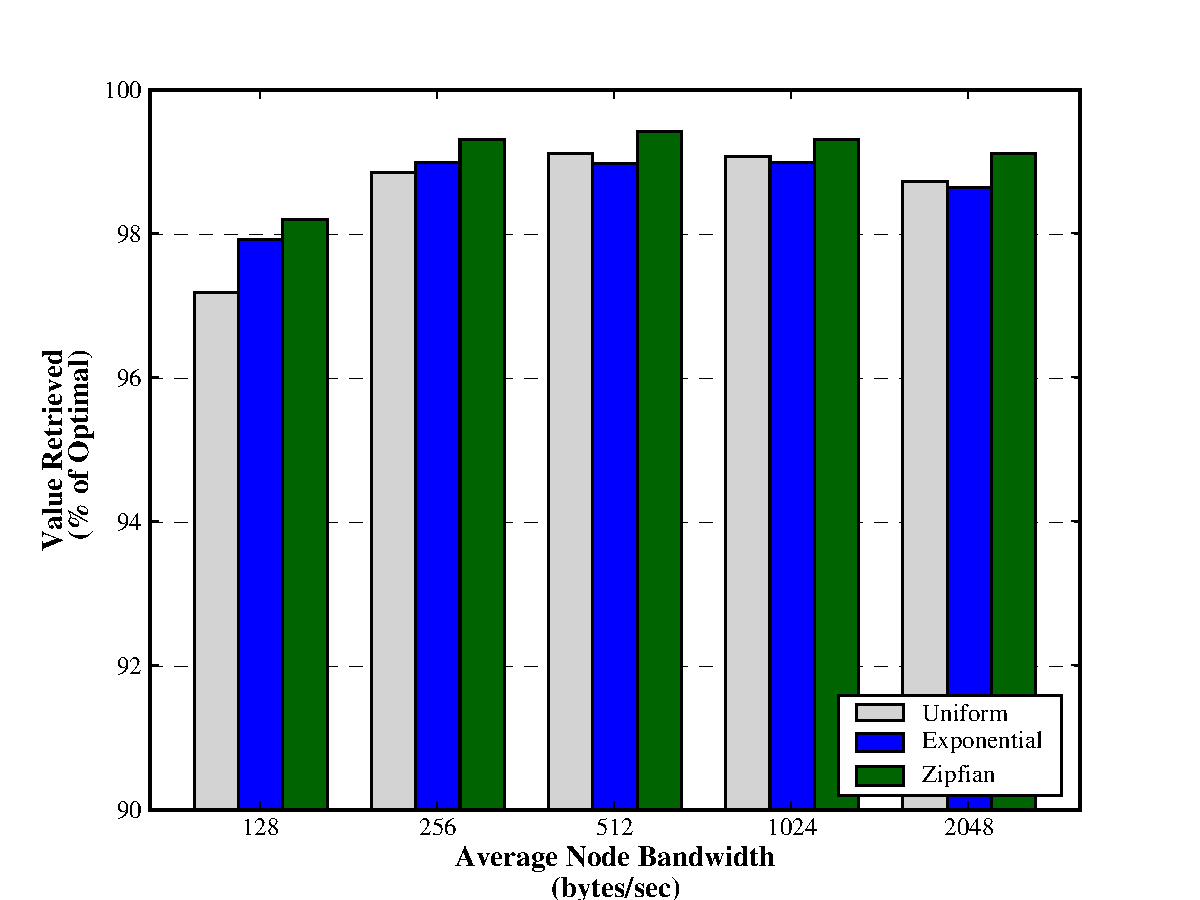
\includegraphics[width=1.0\hsize]{./figs/gwa/speeds/POLICIES.pdf}
\end{center}
\caption{\small {\bf Effect of varying download bandwidth.}
{\em Lance
maintains a high degree of optimality as the per-node download 
bandwidth is varied.
Here results are shown for the three synthetic distributions across a 25~node
tree topology and the \emph{cost-bottleneck} scoring function.  
Note that the $y$-axis starts at 90\%.}}
\label{sec-eval-figspeeds}
\end{figure}


Table~\ref{sec-eval-table} summarizes simulation results from a variety of
different lifetimes and value distributions, run on the 25-node tree
topology. The table shows that the {\em cost-bottleneck} scoring function
outperforms the other two in most cases, with optimality values
between 87.1\% and 96.9\%.
The one exception is the 4-month Zipfian data
set, where \emph{cost-total} slightly outperforms 
\emph{cost-bottleneck}. Figure~\ref{sec-eval-zipfian} shows
the effect of varying the network's target lifetime, using the 
25-node tree topology and a Zipfian data value distribution.
As the figure shows, the \emph{cost-bottleneck} scoring function 
maintains a high degree of optimality as the network bandwidth changes.

To illustrate the effect of varying lifetime targets in more detail,
Figure~\ref{sec-eval-crossover} shows how the optimal solution
transitions between bandwidth-dominant and energy-dominant constraints as the
target lifetime increases. At low lifetime targets, the system is 
bandwidth constrained and cannot download data fast enough to exhaust the 
nodes' batteries.  
At high lifetime targets, the system is energy constrained and
cannot download continuously without exhausting the nodes' batteries.  

\subsection{Bandwidth adaptation} 
\label{sec-eval-params}

Next, we evaluate the impact of varying the download bandwidth in
Figure~\ref{sec-eval-figspeeds}, using the 25-node tree topology and
the \emph{cost-bottleneck} scoring function. We vary the per-node download
bandwidth from 128~to~2048~bytes/s and peg the target lifetime at
8~months. As the figure shows, Lance performs very well
across the range of bandwidths, with optimality greater than
97\% in all cases.

\subsection{Effect of cost vector error}

Our last simulation study evaluates the effect of introducing errors into
estimated download cost. This experiment uses the 25-node topology,
\emph{cost-bottleneck} scoring function, and an exponential data
distribution.  As described in Section~\ref{sec-costassignment}, estimating
the cost of performing different operations {\em a priori} can be difficult.
As shown in Figure~\ref{sec-eval-figerror}, even a 40\% error in each
component of the cost vector $\bar{c}_i$ for a given ADU only degrades
optimality by approximately 15\%. We conclude that accurate estimations
of download costs are not strictly necessary to achieve good performance.

\subsection{Testbed experiments}
\label{sec-eval-policies}

\begin{figure*}[t]
\begin{center}
\begin{tabular}{cc}
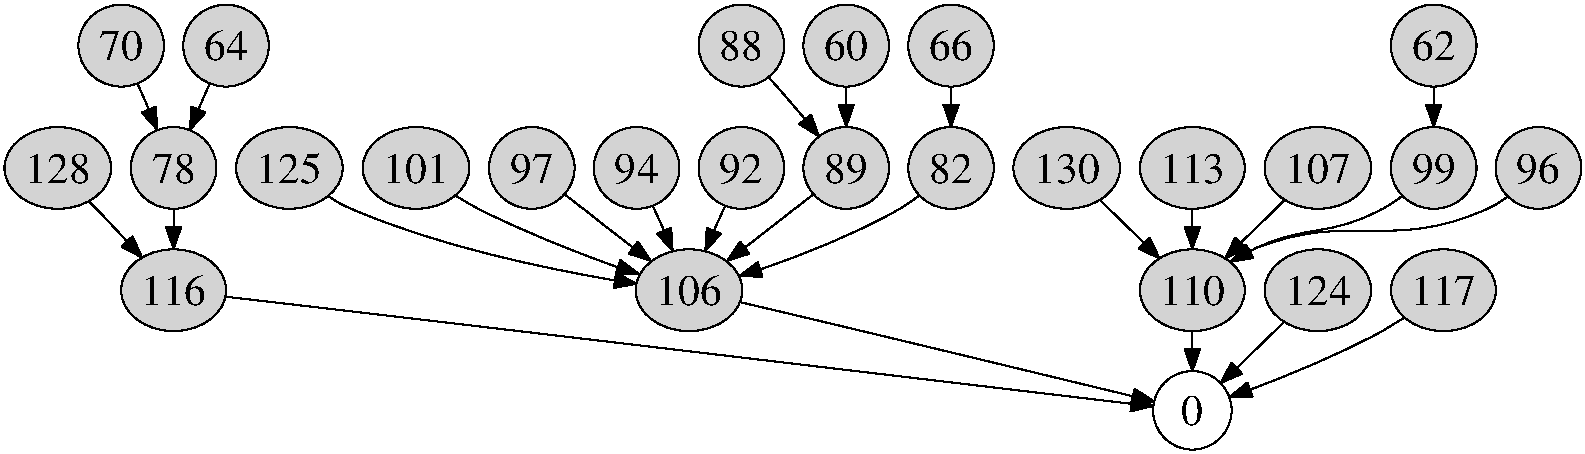
\includegraphics[width=0.45\hsize]{./figs/gwa/topologies/25.pdf} &
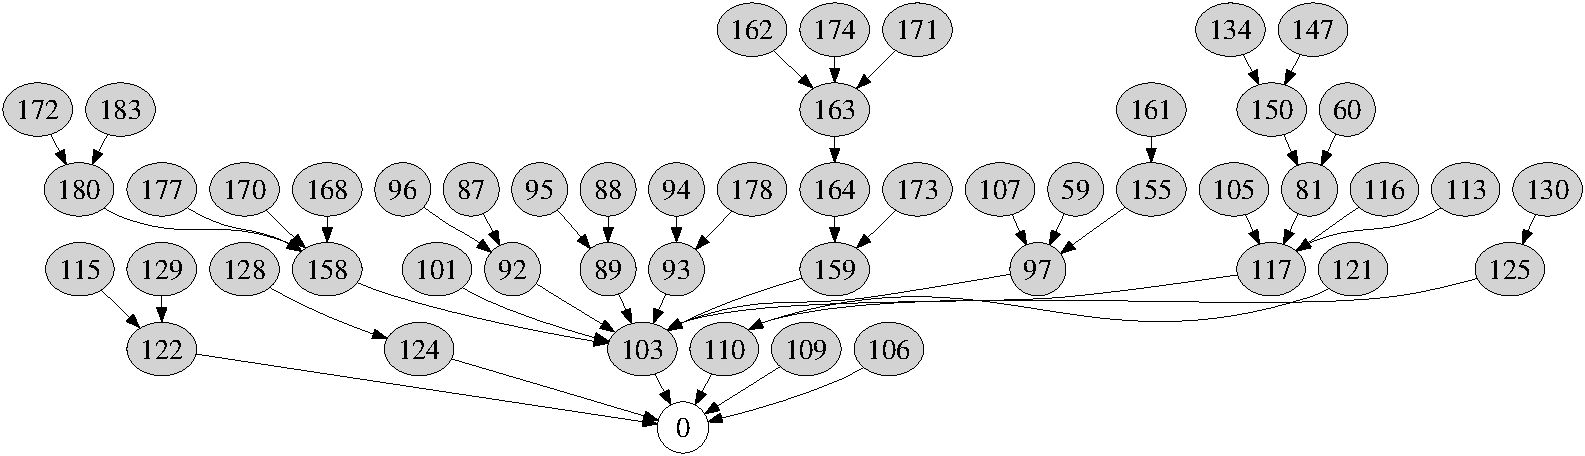
\includegraphics[width=0.45\hsize]{./figs/gwa/topologies/50.pdf} \\
(a) &
(b)\\
\end{tabular}
\end{center}
\caption{\small {\bf Topologies for testbed experiments.} 
{\em This graph shows the 25 (a) and 50 (b) node topologies used for our testbed
experiments.}}
\label{sec-eval-topologies}
\end{figure*}

\begin{figure*}[t]
\begin{center}
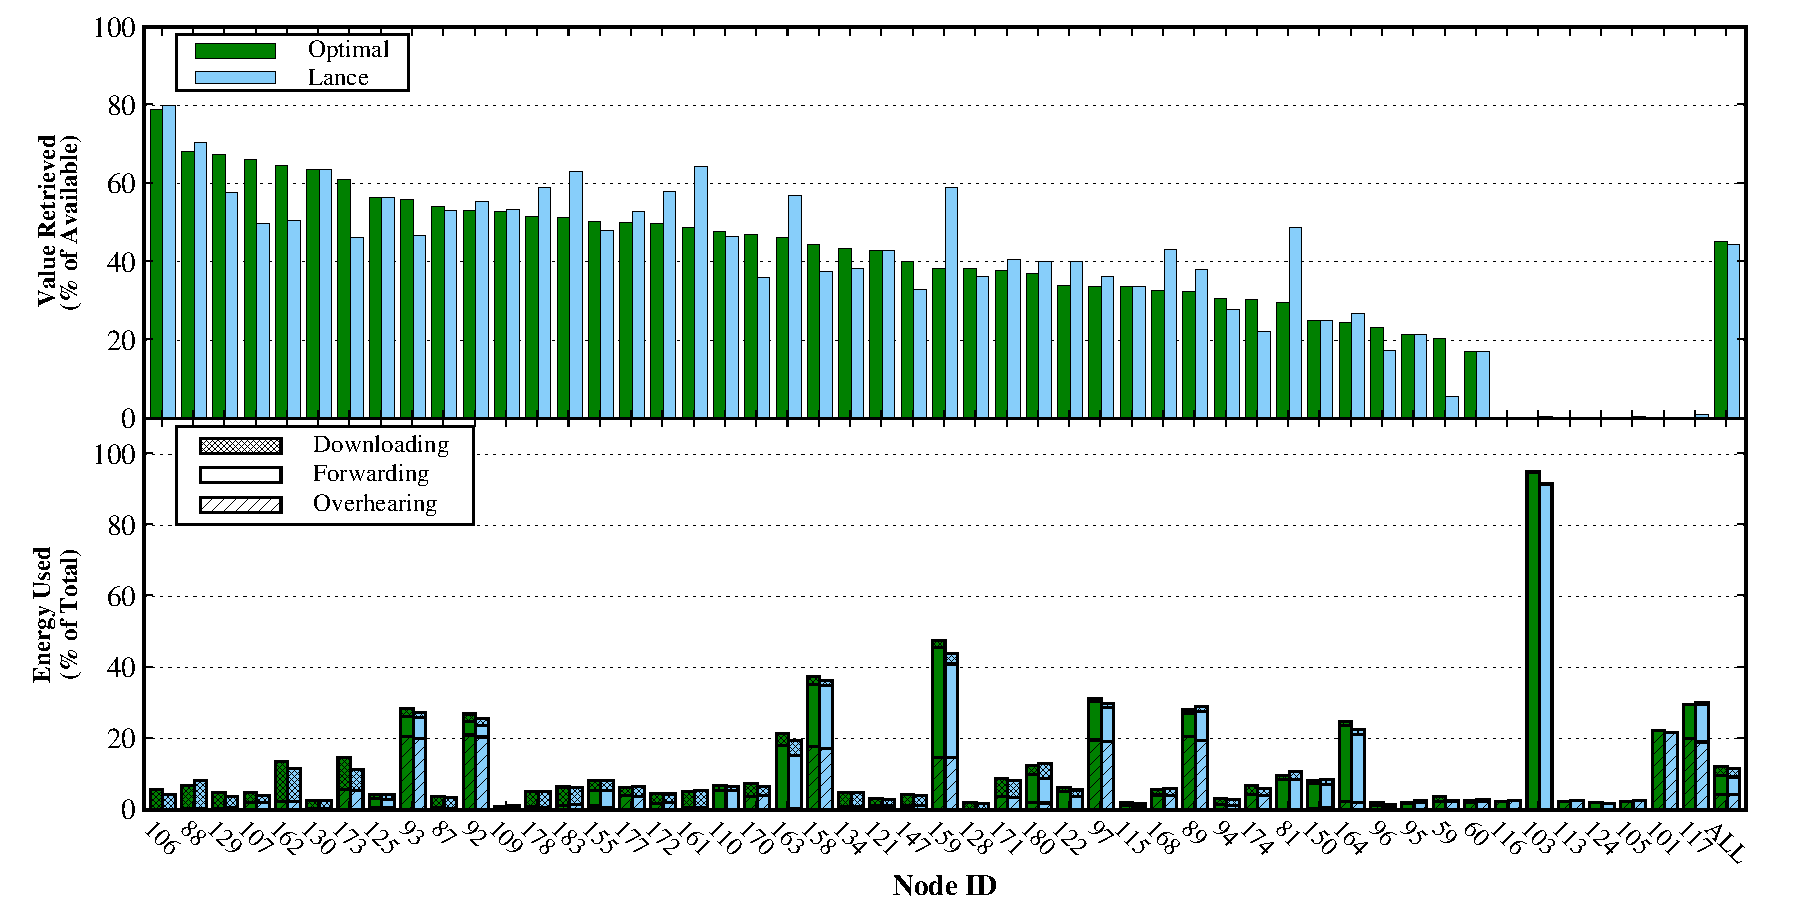
\includegraphics[width=1.0\hsize]{./figs/gwa/big/FIGURE.pdf}
\end{center}
\caption{\small {\bf Optimality and energy use in the 50-node testbed
experiment.} {\em Lance achieved near-optimal performance during 
this 8-hour testbed experiment,
retrieving 98\% of the value obtained by the offline optimal algorithm.}}
\label{sec-eval-figvolcano}
\end{figure*}

In this section, we present results from the Lance system running on the
MoteLab testbed, in 25-node and 50-node configurations shown in
Figure~\ref{sec-eval-topologies}. These experiments stress the system in a
realistic setting subject to radio interference and congestion, and exercise
the multihop routing protocol, Fetch reliable data-collection protocol, and
ADU summary traffic generated by the nodes. For these experiments, we
injected artificial ADU values directly into each node rather than relying on
the nodes sampling real sensor data; this approach allows us to perform
repeatable experiments that explore a wider range of ADU value distributions.
We use the \emph{cost-bottleneck} scoring function. 

Figure~\ref{sec-eval-figvolcano} shows the results of a 50-node testbed
experiment using a Zipfian data distribution and a target lifetime of
6~months.  The upper portion of the figure shows the amount of data value
obtained by Lance from each node, compared to the optimal solution (which was
computed offline). Nodes are sorted by decreasing optimal value. As the
figure shows, Lance achieves very close to the optimal solution, with an
optimality of 98\% overall.  In some cases, Lance incorrectly downloads more
data from some nodes and less data from others; this is due to the inherent
limitations of an online solution that cannot foresee future ADU values.  The
lower portion of the figure shows the energy breakdown for each node with
downloading, forwarding, and overhearing costs shown.  Some nodes consume
more than others because of their location in the routing tree. For example,
node~103 in uses a great deal of energy for routing packets as it is one hop
from the base station, although no ADUs are ever downloaded from that node.

\begin{figure}[t]
\begin{center}
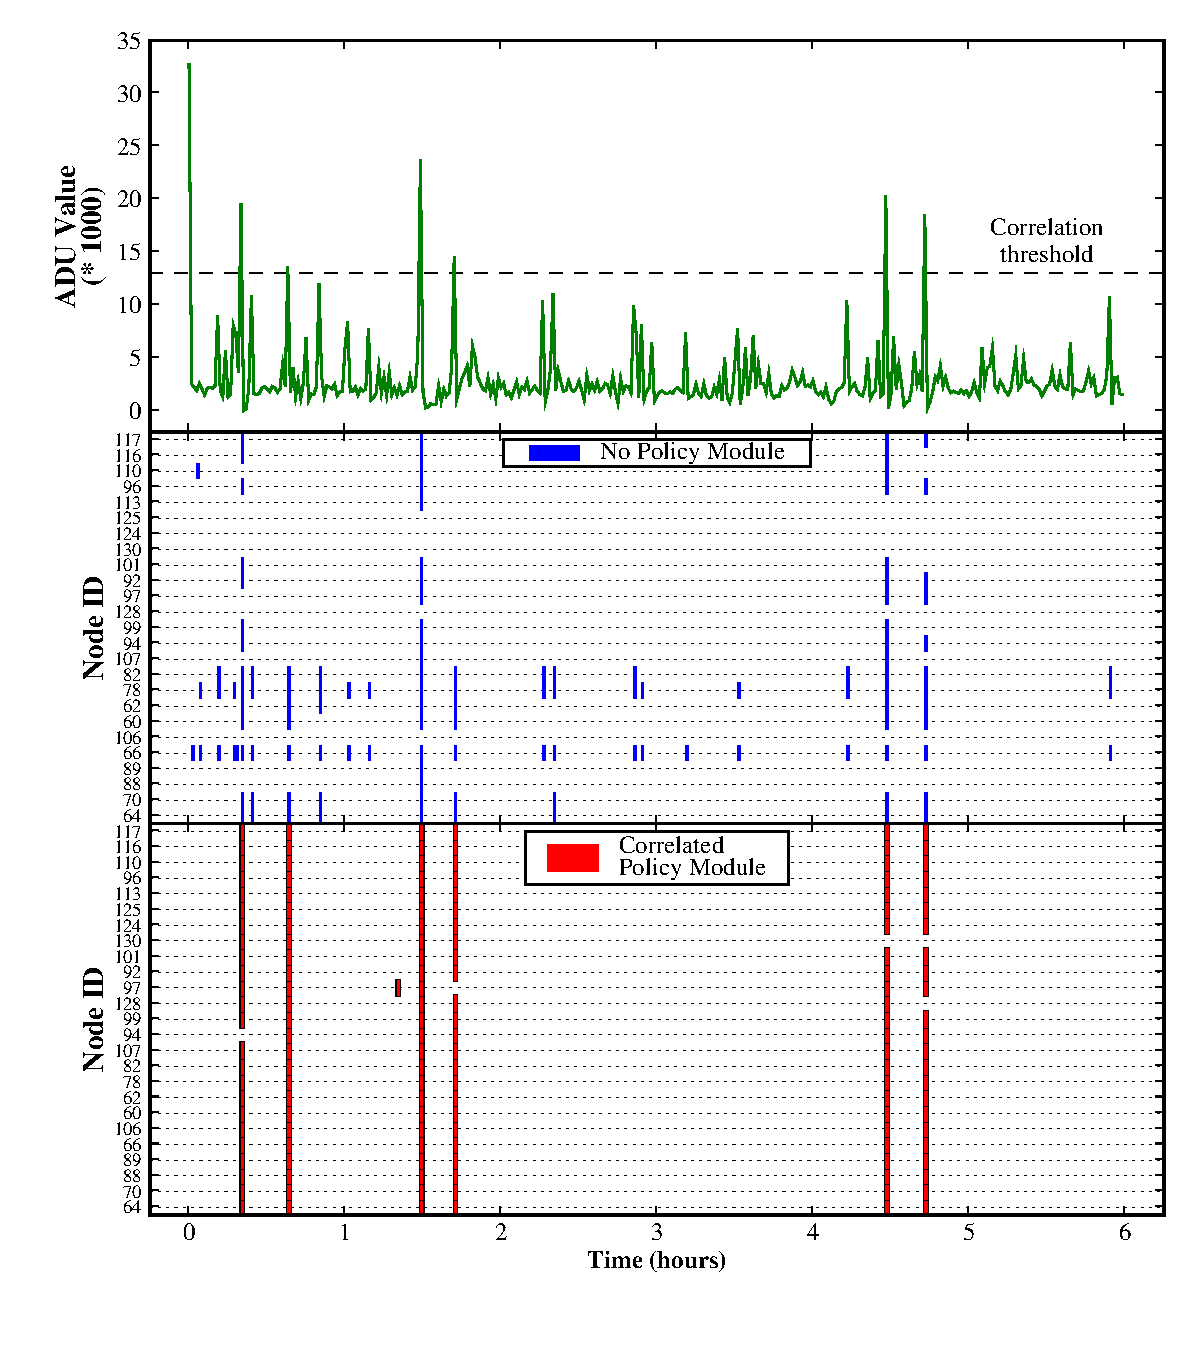
\includegraphics[width=1.0\hsize]{./figs/gwa/policy/FILL.pdf}
\end{center}
\caption{\small {\bf Usage of policy modules to affect download
distribution.} 
{\em Here we illustrate the use of policy modules in the context of
the volcano-monitoring application. The graph compares the download behavior
of the system with and without the policy module chain described in
Section~\ref{sec-ewma-deployment}, which assign greater values to ADUs
corresponding to correlated seismic activity. The graph is colored
at a particular timestamp and node ID if we downloaded that signal from that
node. The top graph shows the ADU values over time, with the threshold for
the \texttt{filter} component of the policy module chain indicated.}}
\label{sec-eval-figpolicyfill}
\end{figure}

Finally, we demonstrate the use of Lance's policy modules.  For this
experiment, we use a distribution of ADU data values based on a 6-hour
seismic trace collected at Reventador Volcano, Ecuador in
2005~\cite{volcano-osdi06}. The raw seismic data is divided into ADUs of 36
KB and ADU values $v_i$ are assigned by computing the ratio of two
EWMA~filters on the data; this assigns greater value to ADUs that contain
earthquakes, as described in Section~\ref{sec-ewma-deployment}. For each node
in the 25-node topology, the ADU values from the seismic trace are attenuated
based on a hypothetical signal source and assigned to each of the 25-nodes
based on their location with respect to the signal source. We then enable a
policy module chain, as described in Section~\ref{sec-policies}, that assigns
higher priority to ADUs that correspond to correlated seismic activity across
the network.

Figure~\ref{sec-eval-figpolicyfill} shows the result of this
experiment running on the MoteLab testbed. The upper portion of the
figure shows the ADU values over time; the middle portion, the set of ADUs
downloaded by the system with no policy modules in use; and the lower
portion, the ADUs downloaded with the policy module chain in use.
As the figure shows, the policy modules cause the network to prefer 
correlated seismic events and download an ADU from all nodes in
the network when such an event is detected. Gaps in the set of ADUs
downloaded are due to download timeouts. In one case, a single ADU 
is downloaded spuriously due to an incorrect value being reported by
that node to the base station. This use of policy modules shows the
drastic change in the system behavior that is affected without
programming the sensor nodes themselves.

\pagebreak
\section{Field Deployment at\\Tungurahua Volcano}
\label{sec-deploy}
\label{sec-deployment}

To evaluate the performance of Lance in a real field setting, 
we undertook a one week deployment of eight~sensor nodes at
Tungurahua Volcano, Ecuador, in August~2007. Lance was used to manage
the bandwidth resources of the sensor network, as
described below. Time and budget constraints prevented us from deploying 
a larger network for longer period of time. 
An earlier version of Lance was used in this deployment
that did not explicitly model energy cost in the download manager. 
However, due to the short duration of the deployment, we knew that 
the battery lifetime used would be more than adequate (two D-cell batteries
offer a lifetime of approximately 12~days with this platform). 
Our primary goal was to validate Lance's operation in a field campaign, 
as well as to identify challenges that only arise in real deployments.

\begin{figure}[t]
\begin{center}
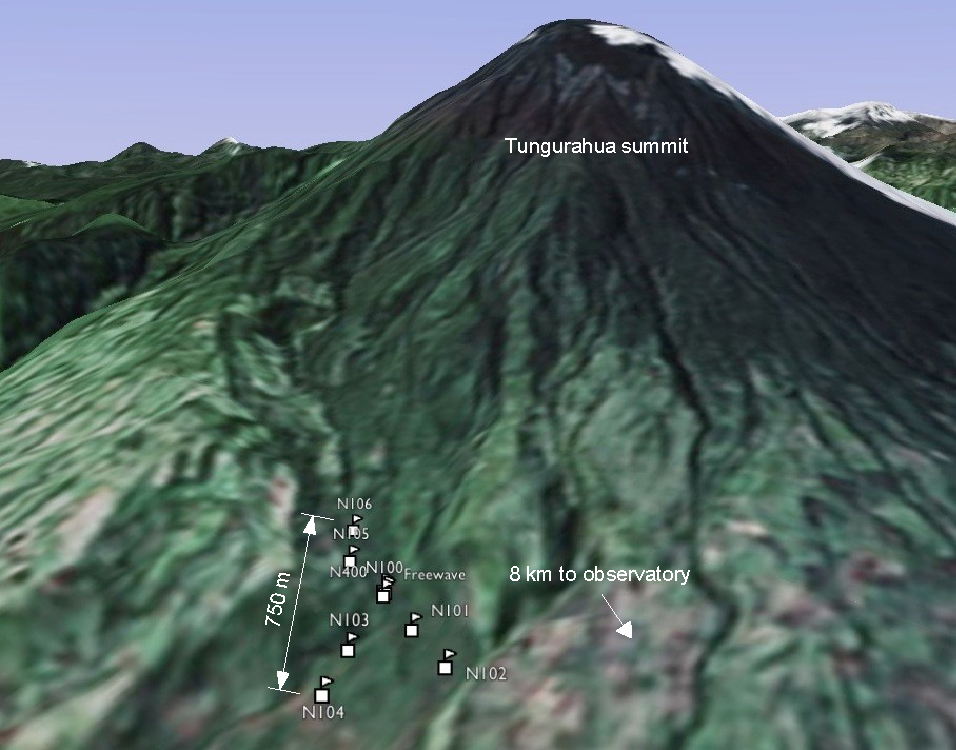
\includegraphics[width=1.0\hsize]{./figs/deploy/deployment-map.pdf}
\end{center}
\caption{\small {\bf Location of the Tungurahua sensor network
deployment.}}
\label{fig-deploy-map}
\end{figure}

The hardware design was based on one used in a previous volcano sensor
network deployment~\cite{volcano-osdi06}.
Each sensor node consisted of a TMote~Sky module
coupled with a custom 24-bit multichannel~ADC board. The network measured
seismic signals using 4.5~Hz geophones and infrasonic signals with small
electret microphones attached to each node.  Data was sampled at 100~Hz
per channel. As shown in Figure~\ref{fig-deploy-map}, seven of the nodes 
were deployed in a three-armed ``star'' topology radiating away from 
a central hub node, with two nodes per arm. 
The eighth node was colocated with the hub and 
transmitted an unreliable continuous stream of sensor data packets 
for establishing ground truth. 
A separate gateway node relayed data (using a FreeWave radio modem) 
to the base station laptop at the volcano observatory, 8~km
from the deployment site. Time synchronization was established using
FTSP~\cite{ftsp} with a single GPS receiver as the root of the
synchronization tree. 
We experimented with two different summarization functions as well as
several different policy modules during the field deployment.

\subsection{Overall performance and data yield}

\begin{figure}[t]
\begin{center}
\begin{small}
\begin{tabular}{|l|l|l|} \hline 
{\bf Node}	& {\bf ADUs downloaded} & {\bf Mean throughput} \\ \hline
100 & 311 & 651.0 B/sec \\
101 & 131 & 446.8 B/sec \\
102 & 262 & 445.8 B/sec \\
103 & 292 & 424.4 B/sec \\
104 & 150 & 256.8 B/sec \\
105 & 66 & 453.7 B/sec \\
106 & 20 & 253.4 B/sec \\ \hline
{\em Total} & 1232 & 431.5 B/sec \\ \hline
\end{tabular}
\end{small}
\end{center}
\caption{\small {\bf Download performance during the deployment.}}
\label{fig-deploy-throughput}
\end{figure}

The sensor network was operational for a total of 71~hours, out of
which the Lance download manager ran for a total of 56~hours. 
During this time, Lance successfully downloaded 1232~ADUs, or 77~MB of 
raw data. An additional 308~downloads failed due to timeout or stale summary 
information, for an overall success rate of 80\%. 
11012~unique ADU summaries were received from the network,
representing an aggregate of 688~MB of sampled data. Lance therefore
downloaded approximately 11\% of the data produced by the network.
Figure~\ref{fig-deploy-throughput} summarizes the number of ADUs
downloaded and the mean throughput for each node. 

\begin{figure}[t]
\begin{center}
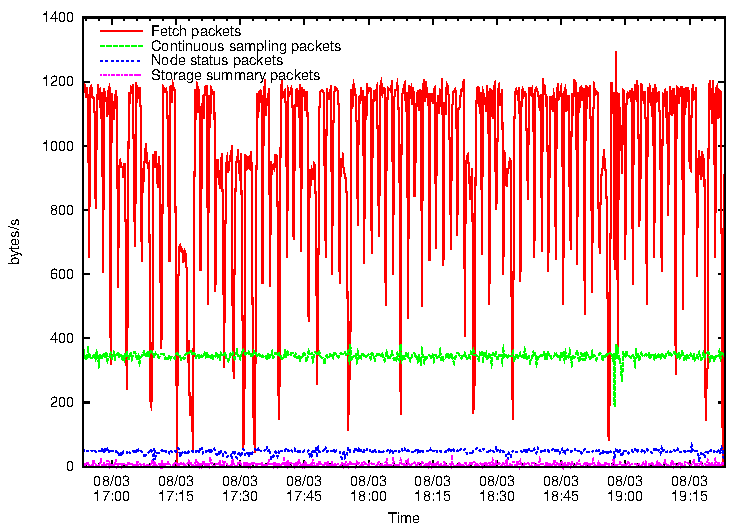
\includegraphics[width=0.9\hsize]{./figs/deploy/packetgraph/packetgraph.pdf}
\end{center}
\caption{\small {\bf Breakdown of radio traffic by packet type.}
{\em This figure shows the total number of bytes received at the base 
station, averaged over 15~sec intervals. Periodic node status messages
and storage summaries comprise a small fraction of the overall
bandwidth.}}
\label{fig-packetgraph}
\end{figure}

Figure~\ref{fig-packetgraph} shows a breakdown of the packets received
at the base station for a representative time period.
Fetch download packets consumed the majority of
the bandwidth, followed by the continuous sampling packets.
The latter is a debugging feature allowing us to visualize the
seismic activity from a single node in real time, and is entirely optional.
Every node sent a periodic heartbeat to the base station every~10~sec,
and a storage summary every 109~sec. As the figure shows, this
overhead is a small percentage (less than 5\%) of the overall network
traffic. 

\pagebreak
\subsection{RSAM-based summarization}

\begin{figure}[t]
\begin{center}
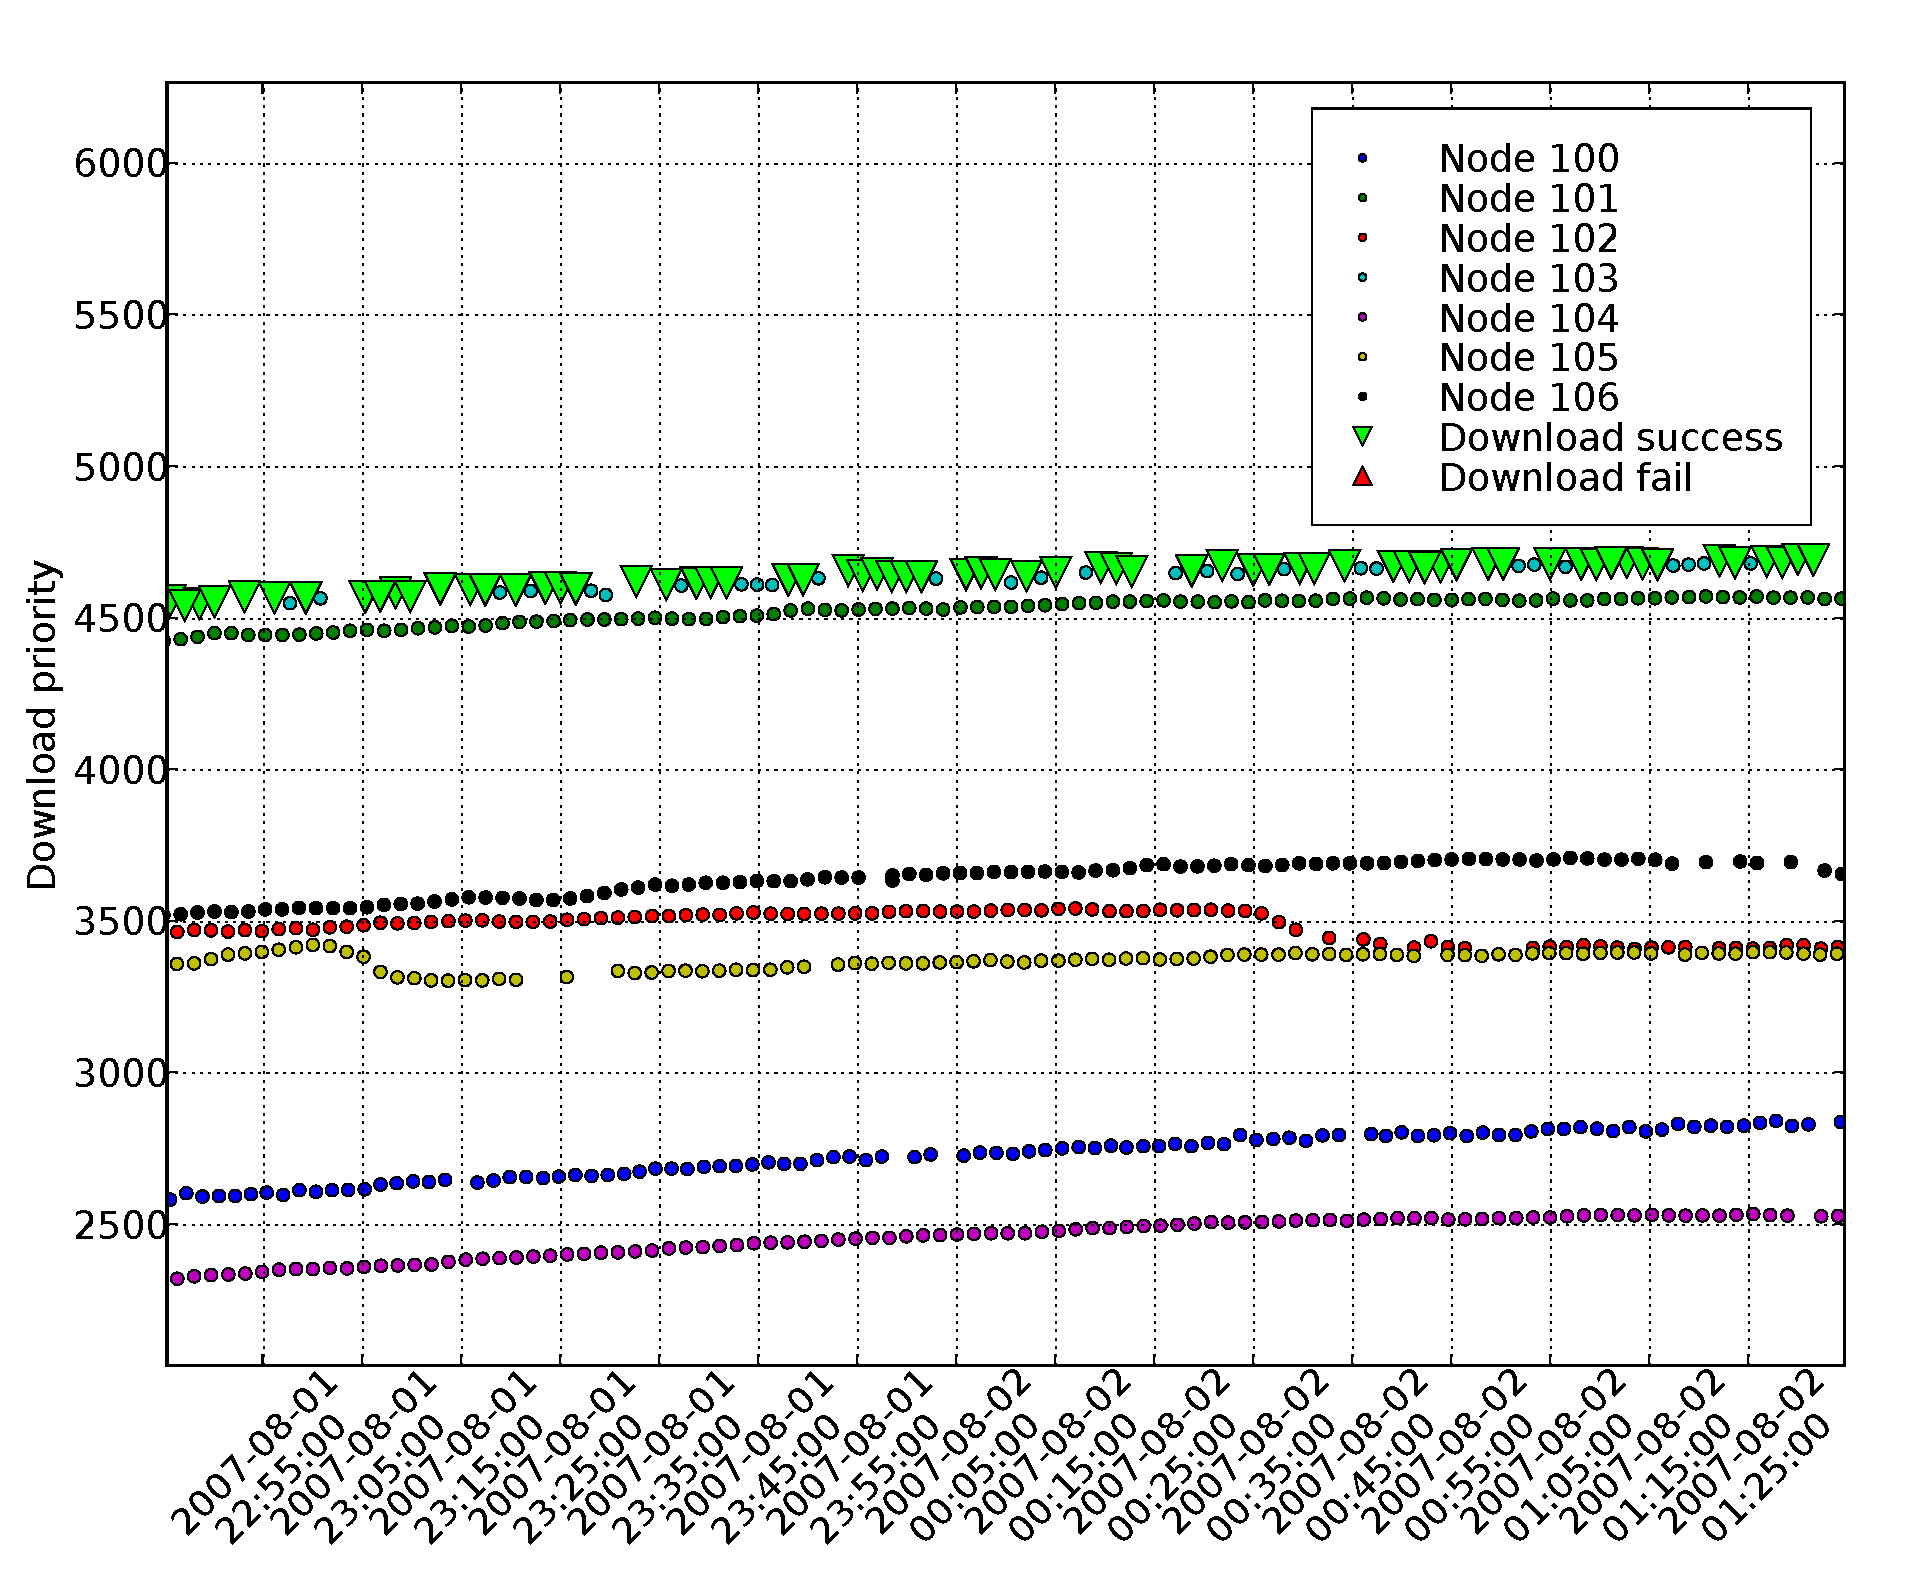
\includegraphics[width=1.0\hsize]{./figs/deploy/downloads-pre-median-filter5.pdf}
\end{center}
\caption{\small {\bf Effect of DC bias on RSAM summarization
function.} {\em Each point represents the ADU value received at
the base station, and the triangles indicate those ADUs that were
downloaded by Lance. Since nodes' RSAM values are
offset significantly from each other, Lance prefers
downloading from the node with the largest positive bias.}}
\label{fig-rsam-dc-bias}
\end{figure}

The system as initially deployed computed the RSAM~\cite{rsam} as the
value for each ADU.
This approach was intended to prioritize data based on
the overall level of seismic activity. We experienced two problems as
soon as the system was fielded. First, the RSAM calculation was
sensitive to DC~bias in the seismometer signal, causing Lance to 
generally prefer downloading ADUs from one or two nodes (those with
the largest positive bias). Figure~\ref{fig-rsam-dc-bias} shows this
effect, with Lance only downloading ADUs from node~103.

This problem was easily corrected, without any node software changes,
by introducing a policy module at the base station to process the 
raw RSAM values received
from each node and filter out the DC~bias. This was achieved by
computing the median RSAM value over each 30-minute window of raw RSAM
values on each node, and subtracting the median from the RSAM.

The second problem with the RSAM summarization function was caused
by the uncharacteristically low level of seismicity at the volcano
throughout the deployment. We observed only about 20~volcano-tectonic 
earthquakes and {\em no} clear explosions, whereas the previous week,
Tungurahua exhibited dozens of earthquakes each day. As a result, the
RSAM summarization function was generally unable to distinguish between
actual seismic activity and noise. We corrected this problem by
switching to a different summarization function (described below)
that was designed to pick out small earthquakes. 

To evaluate Lance's behavior with respect to an ``optimal'' system, we took
the 8483~RSAM summaries received during a 16-hour period when the debiasing
filter was enabled. Using this information, we compute the set of ADUs that
the optimal system would have downloaded, with complete knowledge of all ADUs
but limited to the same time duration the original network was operating.  We
assume the download throughput for a given node is always the mean throughput
for that node observed during the deployment
  (Figure~\ref{fig-deploy-throughput}). This calculation ignores energy
  constraints because the deployed system did not consider energy costs.

An optimal system would have downloaded 392~out of the~8483 ADUs,
whereas the actual system downloaded 418~ADUs during this 
time.\footnote{The optimal system would download fewer ADUs 
than the real system due to the variation in the throughput to each 
node: the optimal system would download more ADUs from nodes 
with lower throughput, thereby limiting the total number of ADUs it could
download.} The total value of ADUs downloaded by the optimal system 
is 10678, whereas the value of the actual network was 10629, for an
optimality of 99.5\%. Lance did an exceptional job of extracting the
highest-value data from the network using our online heuristic
algorithm.

\subsection{EWMA-based summarization function}
\label{sec-ewma-deployment}

Given the low level of volcanic activity, after the first 25~hours of
the deployment we chose to reprogram the network to use a different
summarization function that is designed to pick out small earthquakes
from background noise. This function computes the maximum ratio of two
EWMA filters over the seismic signal; it is similar to that described
in~\cite{volcano-osdi06}. Due to code size limitations on
the motes, it was necessary to manually reprogram each node with the
new summarization function, which took two teams about 4~hours.

This summarization function reports a high value for an ADU
that appears to contain an earthquake or other seismic event. 
However, there is no guarantee that the event will be centered in the
ADU: in the worst case, the earthquake might occur at the very
beginning or very end of the ADU, causing the initial seismic P-wave arrival
or waveform coda to be stored in adjacent ADUs with low value.
To avoid this problem, we made use of the {\tt timespread} policy
module that detects ADUs with
an elevated value (over a fixed threshold) and assigns the
immediately preceding and succeeding ADUs the same value.
By dilating the value over time, Lance should download
all three of the ADUs and maximize the probability that a given
earthquake signal is entirely downloaded.

As with the RSAM-based summarization function, we estimate the optimal set of
ADUs that an oracle would have downloaded. During a 25-hour period, the
network reported 11012~unique ADU summaries. An optimal system would have
downloaded 554 ADUs with total value 577377.  The actual network
downloaded 518~ADUs with a value of 539115, for an optimality of 93.3\%. 

As a final evaluation metric, we wish to consider how well Lance,
configured in this manner, was able to download seismic signals
representing earthquakes. Given the low level of volcanic activity, 
it turns out that most of the ADUs downloaded by Lance contain no 
discernible seismic signal. In fact, upon manual inspection of the
518~ADUs downloaded during this period, we identified only 20~ADUs
showing a clear earthquake signal, corresponding to only 9~separate
seismic events.\footnote{One seismologist remarked that we 
``fixed the volcano'' by placing our sensors on it.}
Note that we did {\em not} configure Lance to explicitly download 
correlated earthquakes as described in Section~\ref{sec-applications},
so we would not expect a high degree of coverage for the same event
across multiple nodes.

\begin{figure}[t]
\begin{center}
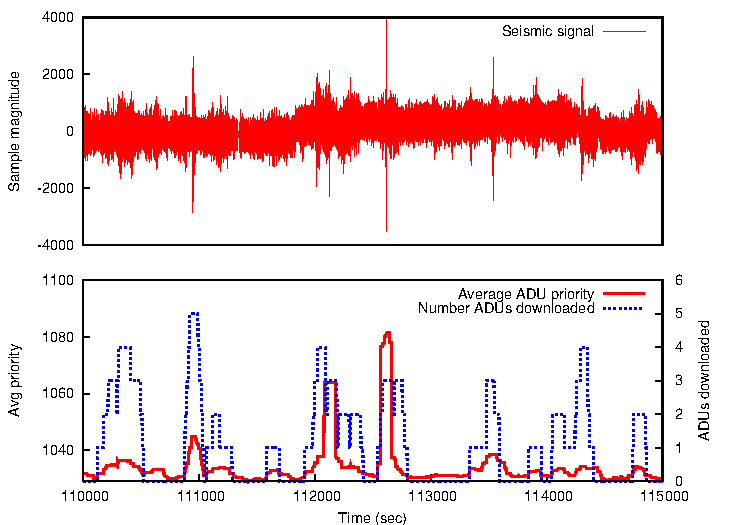
\includegraphics[width=1.0\hsize]{./figs/deploy/deploydownloads/everything.pdf}
\end{center}
\caption{\small {\bf Lance download behavior overlayed with average
ADU value.} {\em The top plot shows the continuous seismic signal
collected by a single node. The lower plot shows the average value
of ADUs and the number of ADUs downloaded for each window.}}
\label{fig-downloads-cont}
\end{figure}

Figure~\ref{fig-downloads-cont} shows the behavior of Lance during a
representative 83-minute period. In the figure, we have broken time
into windows of one-half an ADU duration (55~sec in this case), and
computed the mean ADU value as well as the number of downloaded
ADUs that overlap each time window. As the data shows, elevated seismic
activity is well-correlated with an increase in the ADU value
from across the network, as well as the number of downloaded ADUs.
Moreover, the few cases of clear seismic activity in the trace 
(at times 111000, 112700, and so forth) tend to have more ADUs
downloaded. Of the 9~separate seismic events, a total of 27~ADUs were
downloaded, representing a per-event ``coverage'' of 3~ADUs per event.
This represents just under half of the 7~nodes participating in the network.

\section{Conclusions and Future Work}
\label{sec-conclusions}
\label{sec-conclusion}
\label{sec-future}
\label{sec-futurework}

Lance is intended to address the limited energy and bandwidth resources in
sensor networks by allowing applications to target resource usage at the
highest {\em value} data collected by the network, subject to a lifetime
target.  We have shown that the Lance architecture permits a wide range of
application-specific resource management policies to be constructed atop
several simple underlying mechanisms. Our results show that Lance achieves
near-optimal data retrieval under a range of energy and bandwidth
limitations, as well as varying data distributions. The analysis of our
deployment at Tungurahua shows how Lance can be effective in a field
setting. 

The principles guiding Lance's design also lead to several limitations we
hope to address in future work.  Lance's linear policy modules are easy to
use and compose, although it remains unclear whether more complex
interactions between policy modules are needed. Finally, we hope to study the
use of more sophisticated node-level data processing, including feature
extraction, adaptation to changing energy availability, and data
summarization.  The complications introduced by these features must be
balanced against maintaining the simplicity of our current design.

\subsection*{Acknowledgments}

The authors are indebted to Jeffrey B. Johnson of New Mexico Tech and 
Hugo Yepes of the Instituto Geof\'{i}sico, Escuela Polit\'{e}cnica
Nacional, Ecuador, for their invaluable assistance with the Tungurahua 
volcano field deployment. We also wish to thank our shepherd, Nirupama
Bulusu, for her help with the final version of this paper. This work was 
supported by the National Science Foundation (grant numbers CNS-0546338 
and CNS-0519675) and a generous gift from Microsoft Corporation.

\begin{thebibliography}{10}

\bibitem{cartel}
Cartel.
\newblock \url{http://cartel.csail.mit.edu/}.

\bibitem{aki-richards-80}
K.~Aki and R.~Richards.
\newblock {\em Quantitative Seismology: Theory and Methods}.
\newblock W.H. Freeman, San Francisco, 1980.

\bibitem{girod-ipsn07}
A.~M. Ali, T.~C. Collier, L.~Girod, K.~Yao, C.~E. Taylor, and D.~T. Blumstein.
\newblock An empirical study of collaborative acoustic source localization.
\newblock In {\em Proc. IPSN 2007}, Cambridge, MA, April 2007.

\bibitem{wavescope}
H.~Balakrishnan, S.~Madden, and K.~Amaratunga.
\newblock Wavescope: An adaptive wireless sensor network system for high
  data-rate applications.
\newblock \url{http://wavescope.csail.mit.edu/}.

\bibitem{netshm-spots06}
K.~Chintalapudi, J.~Paek, O.~Gnawali, T.~Fu, K.~Dantu, J.~Caffrey, R.~Govindan,
  and E.~Johnson.
\newblock {Structural Damage Detection and Localization Using NetSHM}.
\newblock In {\em Proc. Fifth International Conference on Information
  Processing in Sensor Networks: Special track on Sensor Platform Tools and
  Design Methods for Networked Embedded Systems (IPSN/SPOTS'06)}, April 2006.

\bibitem{vango}
B.~Greenstein, C.~Mar, A.~Pesterev, S.~Farshchi, E.~Kohler, J.~Judy, and
  D.~Estrin.
\newblock Capturing high-frequency phenomena using a bandwidth-limited sensor
  network.
\newblock In {\em Proc. Sensys 2006}, Boulder, CO, November 2006.

\bibitem{vigilnet}
T.~He, S.~Krishnamurthy, J.~A. Stankovic, T.~Abdelzaher, L.~Luo, R.~Stoleru,
  T.~Yan, L.~Gu, G.~Zhou, J.~Hui, and B.~Krogh.
\newblock Vigilnet: An integrated sensor network system for energy-efficient
  surveillance.
\newblock {\em ACM Transactions on Sensor Networks}, 2004.

\bibitem{tinyos-asplos00}
J.~Hill, R.~Szewczyk, A.~Woo, S.~Hollar, D.~E. Culler, and K.~S.~J. Pister.
\newblock System architecture directions for networked sensors.
\newblock In {\em Proc. the 9th International Conference on Architectural
  Support for Programming Languages and Operating Systems}, pages 93--104,
  Boston, MA, USA, Nov. 2000.

\bibitem{deluge}
J.~W. Hui and D.~Culler.
\newblock The dynamic behavior of a data dissemination protocol for network
  programming at scale.
\newblock In {\em Proc. 2nd ACM Conference on Embedded Networked Sensor Systems
  (SenSys'04)}, November 2004.

\bibitem{ucla-seismic}
A.~Husker, I.~Stubailo, M.~Lukac, V.~Naik, R.~Guy, P.~Davis, and D.~Estrin.
\newblock Wilson: The wirelessly linked seismological network and its
  application in the middle american subduction experiment (mase).
\newblock {\em Seismological Research Letters}, May/June 2008.

\bibitem{shimmer}
{Intel Corporation}.
\newblock {The SHIMMER Sensor Node Platform}.
\newblock 2006.

\bibitem{flush-sensys07}
S.~Kim, R.~Fonseca, P.~Dutta, A.~Tavakoli, D.~Culler, P.~Levis, S.~Shenker, and
  I.~Stoica.
\newblock {Flush: A Reliable Bulk Transport Protocol for Multihop Wireless
  Networks}.
\newblock In {\em Proc. SenSys'07}, 2007.

\bibitem{ggb-ipsn07}
S.~Kim, S.~Pakzad, D.~Culler, J.~Demmel, G.~Fenves, S.~Glaser, and M.~Turon.
\newblock Health monitoring of civil infrastructures using wireless sensor
  networks.
\newblock In {\em Proc. IPSN 2007}, Cambridge, MA, April 2007.

\bibitem{intel-northseasensys}
L.~Krishnamurthy, R.~Adler, P.~Buonadonna, J.~Chhabra, M.~Flanigan,
  N.~Kushalnagar, L.~Nachman, and M.~Yarvis.
\newblock Design and deployment of industrial sensor networks: experiences from
  a semiconductor plant and the north sea.
\newblock In {\em SenSys '05: Proceedings of the 3rd international conference
  on Embedded networked sensor systems}, pages 64--75, New York, NY, USA, 2005.
  ACM Press.

\bibitem{lees-lindley-94}
J.~Lees and G.~Lindley.
\newblock {Three-dimensional attenuation tomography at Loma Prieta: Inverting
  t* for Q}.
\newblock {\em J. Geophys. Res.}, 99(B4):6843--6863, 1994.

\bibitem{enviromic}
L.~Luo, Q.~Cao, C.~Huang, T.~Abdelzaher, J.~A. Stankovic, and M.~Ward.
\newblock Enviromic: Towards cooperative storage and retrieval in audio sensor
  networks.
\newblock In {\em Proc. 27th International Conference on Distributed Computing
  Systems (ICDCS '07)}, June 2007.

\bibitem{wimms-lynch06}
J.~P. Lynch, Y.~Wang, K.-C. Lu, T.-C. Hou, and C.-H. Loh.
\newblock Post-seismic damage assessment of steel structures instrumented with
  self-interrogating wireless sensors.
\newblock In {\em Proceedings of the 8th National Conference on Earthquake
  Engineering}, 2006.

\bibitem{flask-tr}
G.~Mainland, M.~Welsh, and G.~Morrisett.
\newblock Flask: A language for data-driven sensor network programs.
\newblock Technical Report TR-13-06, Harvard University, May 2006.

\bibitem{ftsp}
M.~Maroti, B.~Kusy, G.~Simon, and A.~Ledeczi.
\newblock The flooding time synchronization protocol.
\newblock In {\em Second ACM Conference on Embedded Networked Sensor Systems},
  November 2004.

\bibitem{rsam}
T.~Murray and E.~Endo.
\newblock A real-time seismic-amplitude measurement system (rsam).
\newblock In Ewart and Swanson, editors, {\em Monitoring Volcanoes: Techniques
  and Strategies Used by the Staff of the Cascades Volcano Observatory,
  1980-1990}, volume 1966, pages 5--10. USGS Bulletin, 1992.

\bibitem{netshm-emnets05}
J.~Paek, K.~Chintalapudi, J.~Caffrey, R.~Govindan, and S.~Masri.
\newblock A wireless sensor network for structural health monitoring:
  Performance and experience.
\newblock In {\em Proc. The Second IEEE Workshop on Embedded Networked Sensors
  (EmNetS-II)}, May 2005.

\bibitem{rcrt-sensys07}
J.~Paek and R.~Govindan.
\newblock {RCRT: rate-controlled reliable transport for wireless sensor
  networks}.
\newblock In {\em SenSys '07: Proceedings of the 5th international conference
  on Embedded networked sensor systems}, pages 305--319, 2007.

\bibitem{cyclops}
M.~Rahimi, R.~Baer, O.~I. Iroezi, J.~C. Garcia, J.~Warrior, D.~Estrin, and
  M.~Srivastava.
\newblock Cyclops: in situ image sensing and interpretation in wireless sensor
  networks.
\newblock In {\em SenSys '05: Proceedings of the 3rd international conference
  on Embedded networked sensor systems}, pages 192--204, New York, NY, USA,
  2005. ACM Press.

\bibitem{shooter-localization}
G.~Simon et~al.
\newblock Sensor network-based countersniper system.
\newblock In {\em Proc. ACM SenSys '04}, November 2004.

\bibitem{volcano-ewsn05}
G.~Werner-Allen, J.~Johnson, M.~Ruiz, J.~Lees, and M.~Welsh.
\newblock Monitoring volcanic eruptions with a wireless sensor network.
\newblock In {\em Proc. Second European Workshop on Wireless Sensor Networks
  (EWSN'05)}, January 2005.

\bibitem{volcano-osdi06}
G.~Werner-Allen, K.~Lorincz, J.~Johnson, J.~Lees, and M.~Welsh.
\newblock Fidelity and yield in a volcano monitoring sensor network.
\newblock In {\em Proc. 7th USENIX Symposium on Operating Systems Design and
  Implementation (OSDI 2006)}, Seattle, WA, November 2006.

\bibitem{motelab}
G.~Werner-Allen, P.~Swieskowski, and M.~Welsh.
\newblock {MoteLab: A Wireless Sensor Network Testbed}.
\newblock In {\em Proc. the Fourth International Conference on Information
  Processing in Sensor Networks (IPSN'05)}, April 2005.

\bibitem{zhang2007icedb}
Y.~Zhang, B.~Hull, H.~Balakrishnan, and S.~Madden.
\newblock {ICEDB: Intermittently-Connected Continuous Query Processing}.
\newblock In {\em International Conference on Data Engineering (ICDE)},
  Istanbul, Turkey, April 2007.

\end{thebibliography}
\end{document}
